% arara: xelatex
% arara: xelatex
% arara: xelatex


% options:
% thesis=B bachelor's thesis
% thesis=M master's thesis
% czech thesis in Czech language
% english thesis in English language
% hidelinks remove colour boxes around hyperlinks

\documentclass[thesis=B,english]{FITthesis}[2012/10/20]

% \usepackage[utf8]{inputenc} % LaTeX source encoded as UTF-8
% \usepackage[latin2]{inputenc} % LaTeX source encoded as ISO-8859-2
% \usepackage[cp1250]{inputenc} % LaTeX source encoded as Windows-1250

\usepackage{graphicx} %graphics files inclusion
\usepackage{float}
\usepackage{csquotes}
% \usepackage{subfig} %subfigures
% \usepackage{amsmath} %advanced maths
% \usepackage{amssymb} %additional math symbols
\usepackage{dirtree} %directory tree visualisation
\usepackage{subcaption}

\usepackage[dvipsnames]{xcolor}
\usepackage{listings}

\lstdefinelanguage{Kotlin}{
  comment=[l]{//},
  commentstyle={\color{gray}\ttfamily},
  emph={delegate, filter, first, firstOrNull, forEach, lazy, map, mapNotNull, println, return@},
  emphstyle={\color{OrangeRed}},
  identifierstyle=\color{black},
  keywords={abstract, actual, as, as?, break, by, class, companion, continue, data, do, dynamic, else, enum, expect, false, final, for, fun, get, if, import, in, interface, internal, is, null, object, override, package, private, public, return, set, super, suspend, this, throw, true, try, typealias, val, var, vararg, when, where, while},
  keywordstyle={\color{NavyBlue}\bfseries},
  morecomment=[s]{/*}{*/},
  morestring=[b]",
  morestring=[s]{"""*}{*"""},
  ndkeywords={@Deprecated, @JvmField, @JvmName, @JvmOverloads, @JvmStatic, @JvmSynthetic, Array, Byte, Double, Float, Int, Integer, Iterable, Long, Runnable, Short, String},
  ndkeywordstyle={\color{BurntOrange}\bfseries},
  sensitive=true,
  stringstyle={\color{ForestGreen}\ttfamily},
}


% % list of acronyms
% \usepackage[acronym,nonumberlist,toc,numberedsection=autolabel]{glossaries}
% \iflanguage{czech}{\renewcommand*{\acronymname}{Seznam pou{\v z}it{\' y}ch zkratek}}{}
% \makeglossaries

% % % % % % % % % % % % % % % % % % % % % % % % % % % % % % 
% EDIT THIS
% % % % % % % % % % % % % % % % % % % % % % % % % % % % % % 



\department{Department of Software Engeeniring}
\title{StudyPad - Android Client}
\newcommand{\appname}{StudyPad}


\newcommand{\present}{\begin{minipage}{.1\textwidth}
\centering
      
\includegraphics[width=15pt, height=15pt]{ic_star_black_24dp}
    \end{minipage}}
    
\newcommand{\limited}{\begin{minipage}{.1\textwidth}
\centering
      
\includegraphics[width=15pt, height=15pt]{ic_star_half_black_24dp}
    \end{minipage}}
    
    
\newcommand{\absent}{\begin{minipage}{.1\textwidth}
\centering
      
\includegraphics[width=15pt, height=15pt]{ic_star_border_black_24dp}
    \end{minipage}}
    
\newcommand{\quoting}[1]{\textit{``#1"}}
\newcommand{\fullStar}
	{\begin{figure}[H]
	\centering
  
\includegraphics[scale=0.1]{ic_star_black_24dp.png}
\end{figure}}





\authorGN{Roman} %author's given name/names
\authorFN{Levinzon} %author's surname
\author{Roman Levinzon} %author's name without academic degrees
\authorWithDegrees{Roman Levinzon} %author's name with academic degrees
\supervisor{Ing. Miroslav Bal{\'i}k, Ph.D}
\acknowledgements{THANKS (remove entirely in case you do not with to thank anyone)}
\abstractEN{StudyPad is a combination of a note-taking service and a social network, aimed at helping students to memorise different pieces of information.  The goal of this thesis is to develop an application for Android OS that will serve as the client. This text acknowledges existing solutions, contains domain and requirements analysis, description and the choice of application's architecture and it's implementation.}


\abstractCS{StudyPad je kombinace slu{\v z}by pro pori{\v z}ovan{\' i} pozn{\'a}mek a soc{\'i}{\'a}ln{\'i} s{\'i}t{\v e} s c{\'i}lem  pomoci studentum zapamatovat si ruzn{\'e} informace. C{\'i}lem pr{\'a}ce je vyvinout aplikaci pro OS Android, kter{\'a} bude slou{\v z}it jako klient. Tento text uzn{\'a}v{\'a} st{\'a}vaj{\' i}c{\'i} {\v r}e{\v s}en{\'i}, obsahuje anal{\'y}zu dom{\'e}n a po{\v z}adavku, popis a v{\'y}b{\v e}r architektury aplikace a jej{\'i} implementace}
\placeForDeclarationOfAuthenticity{Prague}
\keywordsCS{Mobiln� aplikace, Android, Kotlin, MVVM, Clean architecture, vzd{\v e}l�v�n�}
\keywordsEN{Mobile application, Android, Kotlin, MVVM, Clean architecture, education}
\declarationOfAuthenticityOption{1} %select as appropriate, according to the desired license (integer 1-6)
% \website{http://site.example/thesis} %optional thesis URL


\begin{document}

% \newacronym{CVUT}{{\v C}VUT}{{\v C}esk{\' e} vysok{\' e} u{\v c}en{\' i} technick{\' e} v Praze}
% \newacronym{FIT}{FIT}{Fakulta informa{\v c}n{\' i}ch technologi{\' i}}

\setsecnumdepth{part}
\chapter{Introduction}

Each year, our smartphones get smarter and mobile applications become more advanced. The arrival of smartphones and mobile applications has completely changed our way of living, made it easier, and it is hard to come up with a single aspect of life, that has not been improved by one or the other application. They are everywhere: helping us to navigate in our neighbourhood, keeping us up to date with latest news, helping us to stay in touch with our loved ones, stay fit and healthy and more. In addition, some of the most popular applications tend to teach us something new.

Educational applications are very popular on both most popular mobile platforms (iOS and Android). Many of them use a flash card system in the study process -- displaying small pieces of information one after another, so that the user can memorise it more efficiently. However, most of these services are fairly limited in terms of what they are trying to teach and some of the greatest  features are scattered across different applications and services. \appname\ is a new solution to this problem. Using Android OS, today's most popular mobile platform, \appname\ wants to give its users freedom in what they can learn and give them proper tools to share, exchange and collaborate on study materials to make the education process even more easier.

\section{Goal}
The goal of this thesis is to deliver  \appname\ client application for  Android OS with the emphasis on content creation, sharing and collaboration. This includes following steps:
\begin{itemize}
	\item analysis of  the existing solutions,
	\item analysis of the functional and non-functional requirements,
	\item requirements design and its implementation,
	\item testing of the resulted solution.
\end{itemize}

\section{Motivation}
The primary motivation is to practice software
development processes on the big and scalable project while applying advanced practices and technics of Android Development. 

\setsecnumdepth{all}

\chapter{State-of-the-art}
\section{StudyPad Service}
\appname\ is a combination of a note taking service and a social network. It is intended for students and everyone who wishes to learn something new. The primary focus of \appname\ is on content creation, its sharing and discovery. 

The \appname\ project originated from several subjects on Faculty of Information Technology (FIT) in Czech Technical University (CTU). The first iteration of backend was introduced as a semestral project for subject Enterprise Java (BI-EJA), and subject Introduction to Android Development (BI-AND) had great influence on the first iteration of the Android Client. All of these components will be described more thoroughly in Chapter 2.

\appname\ core concepts are \textit{Notebooks} and \textit{Notes}. Notebook is simply a collection of notes united by one theme. This may be a subject in school, a language that you would like to learn or a set of questions that you could hear at a job interview. Note, in turn, is a part of the notebook and represents a single piece information that has a name and a content. It can also be interpreted as a question and answer or a term and its definition.


Each user has his/her own space where they can create, store and edit notebooks and notes (hereafter \textit{Library}). All notebooks stored in the library can be used in various tests and exercises to help users to memorise its content.
\subsection{Sharing \& Collaboration}
\appname\ also allows users to easily share their notebooks with each other. Each notebook can be shared by creating a published version of it (hereafter Published Notebook),thereby making it available to everyone else for viewing and importing.
The publication process involves providing additional information about the notebook, including its name, an optional description, topic and optional tags that serve to narrow the topic. Everything the user has provided(hereafter Author) along with their school and language will then be used in the process of searching and filtering -- which will facilitate the search for the necessary materials. \appname\ also makes it possible to quickly share a notebook by sending a link, which will act as a deep-link, navigating the user directly to a Published Notebook.

The Author of the notebook reserves the right to make edits/corrections to the Published Notebook. Other users (hereinafter subscribers) in turn can save a Published Notebook to their library or suggest some changes or corrections to improve the content. By saving Published notebook to his/her library, the subscriber will be able to make any local changes as he/she sees fit and use it as normal. The Subscriber will be notified about any updates made to the Published Notebook so that he/she can apply the changes to his/her local version, however, any local changes will be deleted. The Author of the notebook, in turn, will be notified about latest suggestions and comments left by the subscribers.


\begin{figure}[H]
\centering
  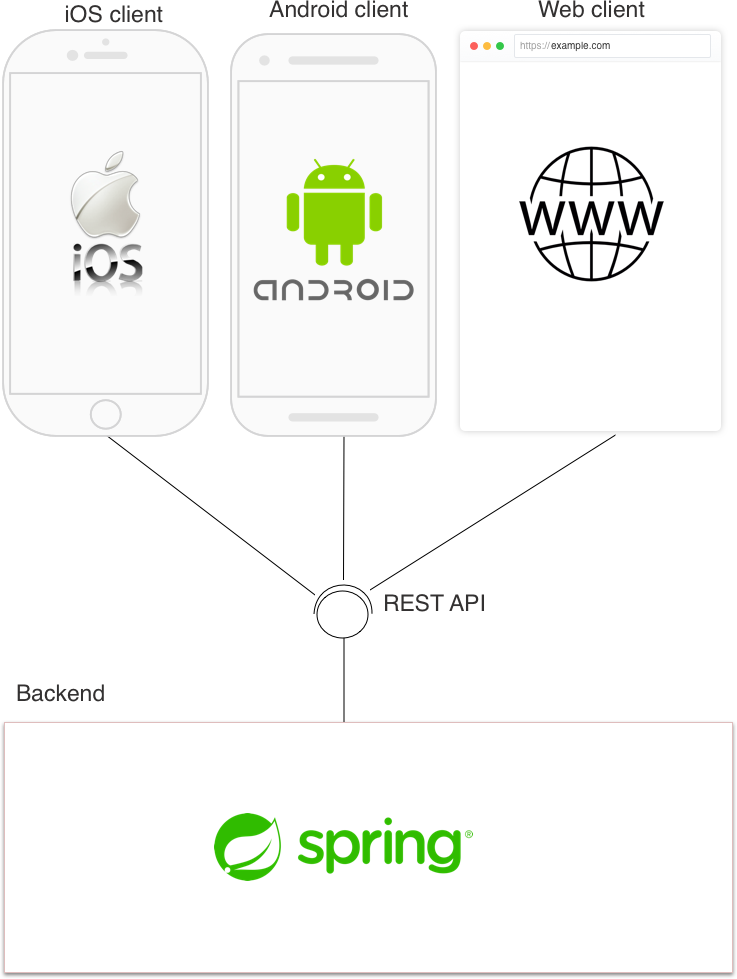
\includegraphics[scale=0.26]{systemdesc}
  \caption{\appname\ sevice}
  \label{fig:android-component}
\end{figure}




 
	\section{Android Platform}
Android is a mobile operating system developed by Google. It is based on a modified version of the Linux kernel and other open source software, and is designed primarily for touchscreen mobile devices such as smartphones and tablets.\cite{android-platform}



\subsection{Android SDK Versions}
Since its inception, several versions have been released, with the latest one being 9.0, codenamed \enquote{Pie}. Every new version provides new and improved APIs to work with and backward compatibility for applications running on older versions.\cite{android-sdks} Originally, the Support Libraries were used to provide backward compatibility while targeting newer versions. This was the case until AndroidX was introduced.

AndroidX, in essence, is a refactored version of the Support Libraries. Just like Support Libraries it ensures backward-compatibility and is shipped separately from the Android OS, but it also provides a more clear and convenient package names and uses a strict semantic versioning system. \cite{androix-overview}

When developing applications for Android, the developer has to consider which OS versions the application will support. Specifically, the \texttt{minSdkVersion} and \texttt{targetSdkVersion} attributes are used to identify the lowest API level with which your application is compatible and the highest API level against which you have designed and tested your application. \appname\ will target the latest Android version available, with the minimal version set to 5.0, codenamed Android Lollipop. This will ensure a high compatibility rate of 85\% and Material Design Support, which is one of the non-functional requirements.


\begin{figure}[H]
\center
  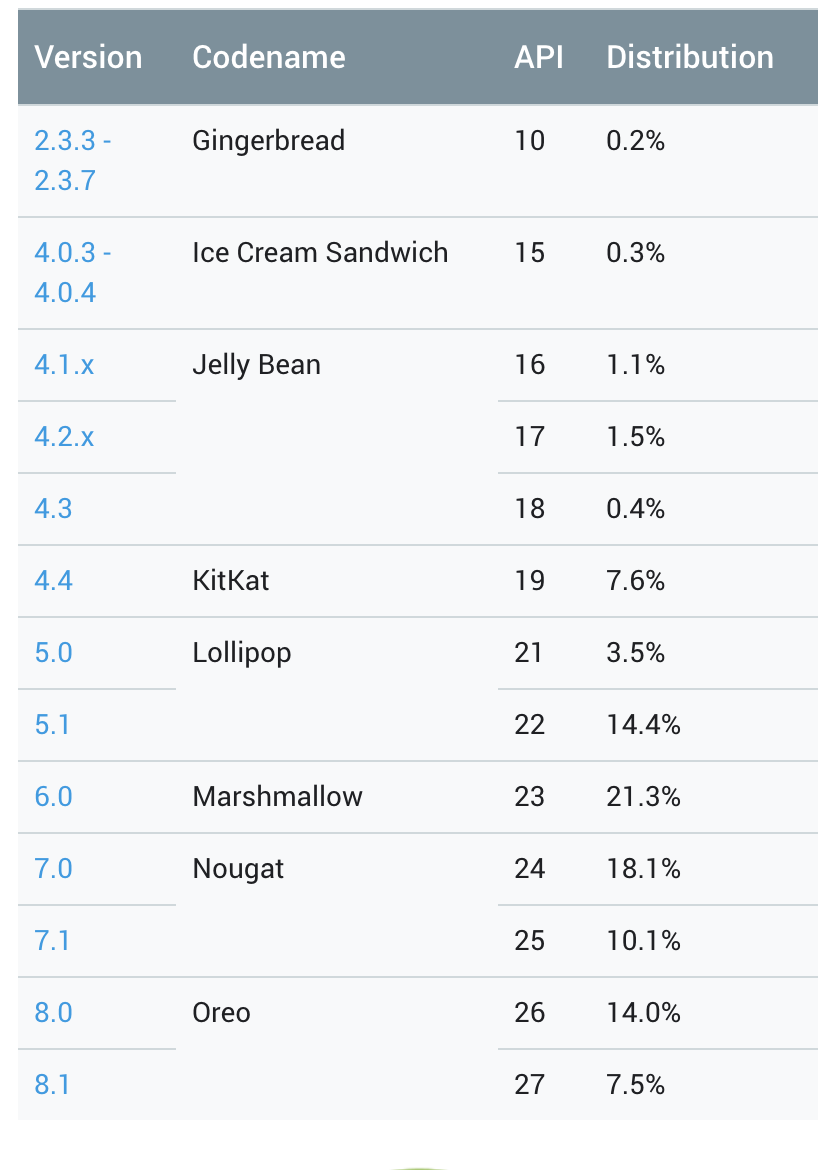
\includegraphics[scale=0.5]{adnroidversion.png}
  \caption{Android Versions distribution}
  \label{fig:androidversions}
\end{figure}

\subsection{Android High-level Framework Elements}
Android SDK provides multiple elements and APIs for developers to help them build UI and communicate with the Android OS.
\begin{itemize}
	\item \textbf{Activity}: \texttt{Activity} represents a single window where the UI elements can be placed. Android OS managing the creation and destruction of the \texttt{Activities}, that is why \texttt{Intents} are used to start/launch it. Activity's lifecycle is  \cite{android-activity}. 
	\item \textbf{Fragment}: \texttt{Fragments} were introduced in Android 3.0, primarily to support more flexible UI designs for larger screens (like Tablets). In such designs, \texttt{Activity} serves as container for one or more \texttt{Fragments}, and because each \texttt{Fragment} defines its own layout with its own lifecycle, it can be used in multiple  \texttt{Activities} \cite{android-fragment}.
	\item \textbf{Broadcast Receiver}: \texttt{Broadcast Receiver} allows the application to receive and send local and system-wide broadcasts similar to the publish-subscribe design pattern. By using \texttt{Broadcast Receiver} application can act upon receiving various kind of events, like the change of internet connectivity or charging status.\cite{android-broadcast}.
	\item \textbf{Service}: \texttt{Service} is the application component that does not require UI and is used to perform long-running operations, even if the user stops interacting with the application \cite{android-service}.
	\item \textbf{Intent}: \quoting{An intent is an abstract description of an operation to be performed}. \texttt{Intent} can be used to launch an \texttt{Activity}, start a \texttt{Service} or a \texttt{BroadcastReceiver}. \texttt{Intent} can either start a specific component (explicit Intent) or try to find a component that can complete certain actions (implicit Intent) \cite{android-intent}.For example,  there could be several applications available on the device with the image viewing functionality, implicit intent, in this case, will allow the user to choose which application will handle this section. Explicit intent, on the other hand, is perfect when launching your own \texttt{Activities} and other components. 
	\end{itemize}
	
	
	\subsection{Resources}
Resources are the additional files and static content that your code uses, such as bitmaps, layout definitions and user interface strings. Resources are stored in the separated package called \texttt{/res} and can be referenced in the application using ids. Also, depending on current configuration, Android can choose appropriate resource version (if multiple are provided) at run-time. For example, it can be used for localisation support by providing different strings resources for different languages.\cite{android-resources}
	
	\subsection{Views} 
	
	\texttt{View} is fundamental building block for all the UI components. It serves as base class for \texttt{Widgets}, which are the interactive elements and \texttt{ViewGroups}, that acts as a containers for other Views. \cite{android-views}
	
	\texttt{ViewGroup}, as mentioned before, is an invisible container that holds other views. Android provides different ViewGroup subclasses, each with its own purpose and a way to structure its children \cite{android-viewgroup}. \texttt{LinearLayout}, for example, allows to align widgets horizontally or vertically.\cite{android-linear}. Another important ViewGroup that has received a lot of attention and support during the last couple of years is ConstraintLayout. Using constraints, it allows developers to create more complex layouts without using nested ViewGroups (i.e., LinearLayout inside another Linear Layout).\cite{android-constraints}
	
	Android uses XML for declaring the UI for Activities and Fragments. XML is then converted to the View object using \texttt{LayoutInfalter}.  Views can also be added programmatically via Java/Kotlin code.	

\section{Android Studio}
Android Studio is an official IDE for Android development. Out of the box it provides a lot of essential tools, like visual Layout editor, emulator and more. 


\section{Gradle}
Gradle is a build toolkit, that is used to automate and manage the build process, while allowing you to define flexible custom build configurations using Groovy-based DSL (Domain Specific Language). Android plugin, shipped alongside the Android Studio, allows to modify and control various build parameters such as \texttt{buildVariant}, dependencies, artifacts signings, and manifest entries.\cite{android-gradle}

\section{Kotlin}
\quoting{Kotlin is a pragmatic programming language for JVM and Android that combines OO and functional features and is focused on interoperability, safety, clarity and tooling support.} Kotlin is a general purpose language developed by JetBrains and it works everywhere Java works and is fully interoperable with it, meaning every Java code can be converted to Kotlin and vice-versa.\cite{kotlin} Since May 17th 2018, Kotlin became the official language for Android development with all the tools and libraries required shipped with Android Studio out of the box.\cite{kotlin-android}. 


\subsection{Kotlin Extensions}
Similar to some other languages, Kotlin provides a way to extend any class with new functionality without inheritance. There are two types of extensions: Functions and Properties. All the extensions are resolved statically and do not modify the class they extend.\cite{kotlin-exts}

When it comes to Android, a  plugin developed by JetBrains provides a lot of useful extensions that enhance the experience of Android development. For example, it is possible to reference Views from Activity/Fragments directly using its ids. Previously it was required to call \texttt{findViewById<View>()} (Listing \ref{code:viewbinding}) to obtain a view reference, which resulted in a lot of boiler-plate code. \cite{kotlin-androidexts}


 \begin{lstlisting}[caption={Kotlin View Binding example}, label={code:viewbinding}, language=Kotlin]
   // Instead of findViewById<TextView>(R.id.textView)
   textView.setText("Hello,world!")

\end{lstlisting}



Due to its official support and features, Kotlin was chosen as a primary language for \appname\ development as opposed to Java.

\section{Application Architecture}
Application Architecture defines the way different application elements interact with each other and how the application is designed and organised. 

\subsection{Clean Architecture}
Clean architecture is a set of ideas derived from different kinds of other approaches with the main principle being a separation of concerns. 
Separation of concerns ensures that all the application's components are easily replaceable and as less independent as possible. When it comes to Android and every software that contains UI, it is essential that the UI does not contain any business logic and serves only as a way to show information.


\subsection{MVP}
MVP or Model-View-Presenter is an architecture pattern that is very common in Android development. 
Model is the data layer
View is the UI layer, which in the Android worlds are Fragments and Activities. 
Presenter - is the layer between the View and the Model. It receives events from the View and updates the Model layer and applies the result to the UI layer.
The View and Presenter both are abstracted to an Interface, it makes all the layers easily testable. \cite{arch-mvp} However, one of the main disadvantages is that Presenter must hold a reference to a View, which can lead to memory leaks and other problems around Android lifecyle.

\subsection{MVVM}
MVVM or Model-View-ViewModel is another pattern to apply Clean Architecture principles. It is very similar to MVP  when it comes to View and Model layers, with the only difference being ViewModel.
ViewModel, as oppose to Presenter, is not aware of the View -- it does not hold the reference to it. Instead, View subscribes to ViewModel events and its state accordingly. ViewModel handles UI interactions, updates the Model layer and then post changes so that the View can get updated.\cite{arch-mvvm}

\subsection{Android Architecture Components}
Previously, Google, as the leading Android contributor, never cared about the way developers build their applications. It has changed drastically with the introduction of Architecture Components at Google I/O in 2017.\cite{android-archcomponents}
Architecture Components are a collection of libraries that can be used to design a robust and maintainable architecture.  LiveData and ViewModel components are the most important.  LiveData is a lifecycle-aware component is used to store data and notify its subscribers if the data changes.  ViewModel can store UI-related data and survive Activity Destruction which is especially useful in case of device rotation for example.

\subsection{Recommended Architecture}
Introduction of Architecture Components made it clear what approach Google recommends when designing application architecture - MVVM. Figure \ref{fig-arch} demonstrates this approach:
\begin{itemize}
	\item Fragments and Activities represent the View
	\item View is connected to a ViewModel. ViewModel there is represented by a ViewModel Architecture component that stores model data using LiveData, that Fragment or Activity can subscribe to. ViewModel requests data from the repository, without knowing where the data comes from
	\item A Repository pattern represents the Model layer. Repository's responsibility is to retrieve and modify the data using one or multiple sources. Typically there is remote data source (API) and the local data source (on-device database).
\end{itemize}

\begin{figure}[H]
	\centering
  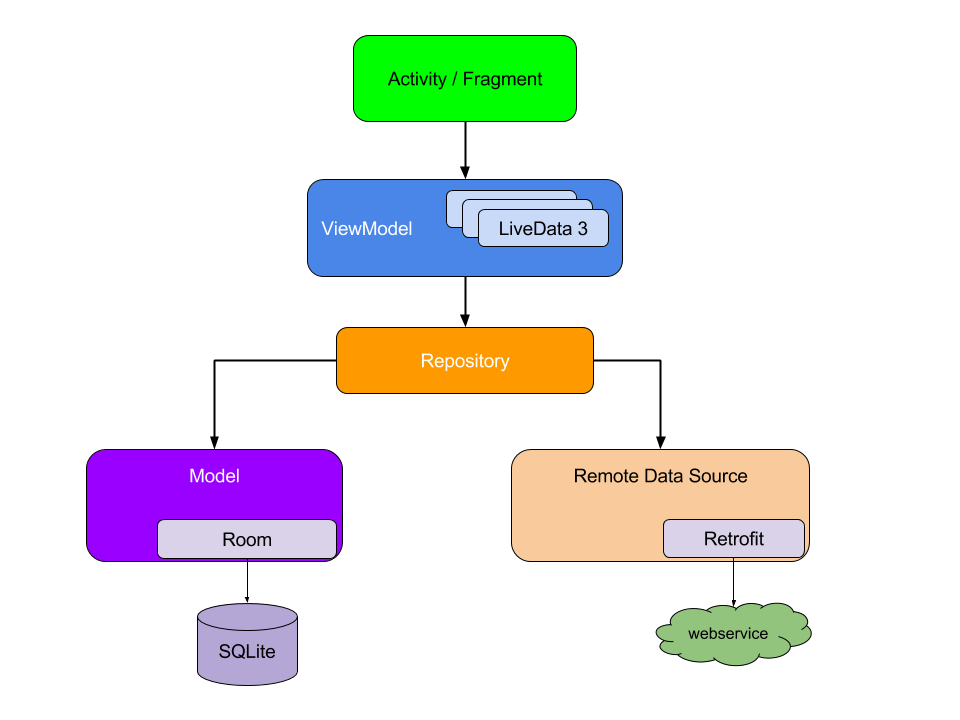
\includegraphics[scale=0.4]{final-architecture}
  \caption{Architecture Example Diagram}
  \label{fig-arch}
\end{figure}


\subsection{Chosen Architecture}
The fact that the MVVM  pattern is recommended by the developers of the Android OS and the existence of Architecture Components makes MVVM a solid choice and good starting point for the application architecture. Its detailed design and implementation is discussed in the following chapters.




\section{Firebase}

\quoting{Firebase lets you build more powerful, secure and scalable apps, using world-class infrastructure.} \cite{firebase} Firebase provides a high number of services, some of which are a necessity in today's world of software development. \\\appname\ will be using the following services:
\begin{itemize}
	\item \textbf{Firebase Analytics} Firebase Analytics provides free application measurement solution, that allows you analyse how the users interact with your application based  on up to 500 distinct events \cite{firebase-analytics}
		\item \textbf{Firebase Cloud Messaging} \quoting{Firebase Cloud Messaging (FCM) provides a reliable and battery-efficient connection between your server and devices that allows you to deliver and receive messages and notifications on iOS, Android, and the web at no cost.}\cite{firebase-messaging}
	\item \textbf{Firebase Auth} \quoting{Firebase Auth  provides an end-to-end identity solution, supporting email and password accounts, phone auth, and Google, Twitter, Facebook, and GitHub login, and more.}\cite{firebase-auth}
	\item \textbf{Crashlytics} Crash Reporting allows you track detailed reports of the errors and crashes in the application. All the issues experienced by the users are then grouped into clusters of similar stack traces and triaged by the severity of impact on application users.\cite{firebase-crash}

\end{itemize}.

\noindent While Firebase Analytics and Crash Reporting services are a great help while developing mobile applications, Firebase Auth and FCM are essential for some of the functional requirements. 

Storing user credentials, and most importantly, storing them safely is not an easy task. With a little effort, Firebase Auth will handle everything related to user management, including access token generation and refreshment, as well as credentials storing and encryption.

Firebase Cloud Messages will enable push-notifications, which is a great way to interact with users and introduce some real-time functionality to the application. 



\section{Material Design}
Material Design is a design language that Google developed in 2014. Later in 2018, it was revamped with a goal to provide more flexibility for designers to create more custom themes. Material Design was chosen as a main source of inspiration when creating \appname\ UI due following  reasons:
\begin{itemize}
	\item Material Design has very wide support on Android Platform. Every component that is described in Material Design Guidelines is implemented by Google and can be used by developers.
	\item Material Design is cross-platform, meaning that its guidelines can easily be applied when creating design for other platforms like iOS or Web.
\end{itemize}
\chapter{Analysis}
This chapter contains a \appname\ system description and analysis with the goal to identify requirements and how it compares with its rivals

\section{System description}

The \appname\ system follows classic client-server software architecture. The server part is represented by the Spring Boot application, which communicates with its clients using REST API. The client part consists of client applications for several platforms: Android, iOS and Web. The Web client is being developed alongside the Android client to serve as an Admin Panel.\cite{studypad-web} The iOS client was developed by the author of this thesis  within the subject Introduction to iOS Development (BI-IOS). \cite{studypad-ios} The main task of this thesis is to deliver an Android OS client.

\subsection{User Roles}
Some of the use-cases requires moderation. The simplest example is a university creation use-case. Though it is possible to submit new school/university in case user haven't found it, the name, that user has submitted has to be verified first and other details, like school location and translations should be updated. This is a main purpose of the Admin Panel and it will require an introduction of different user roles: User and Admin. 

The User role is a default one and will be assigned automatically to everyone who completes the registration process. It will only be used in the client applications.
Admin role is the only one that have the access to the admin panel and an ability to view and modify certain data.

\subsection{\appname\ API}
\appname\ has its own REST API that is represented by Spring Boot application using JSON as a data-interchange response format. \cite{studypad-backend} The Spring Framework is a Java-based framework that enhances developing of Java EE applications. It has modular architecture and supports Dependency Injection and using Inversion of Control principles.\cite{wiki-spring}. In Spring 5.0 official support for Kotlin has been introduced.\cite{spring-kotlin}


The author of this thesis developed the first iteration of the API as a semestral project for subject BI-EJA. The API is still being updated to support requirements for the client applications.
\subsection{Android client}

The detailed structure of the Android client and how it is connected with other components is presented on the component diagram on Figure \ref{fig:component}. 

 Android component will be divided into three layers: the Data Layer, Business Layer and Presentation layer. The Data layer is only responsible for downloading and storing data. The Business Layer responsibility is to handle user interactions and converting downloaded data to something that presentation layer can present. Presentation layer is only responsible for displaying data. Android component will also connected be to Facebook SDK, Google Auth SDK and Firebase SDK to provide authentication options. Firebase SDK will also enable an analytics service, crash reporting and push notifications.


\begin{figure}[H]
\centering
  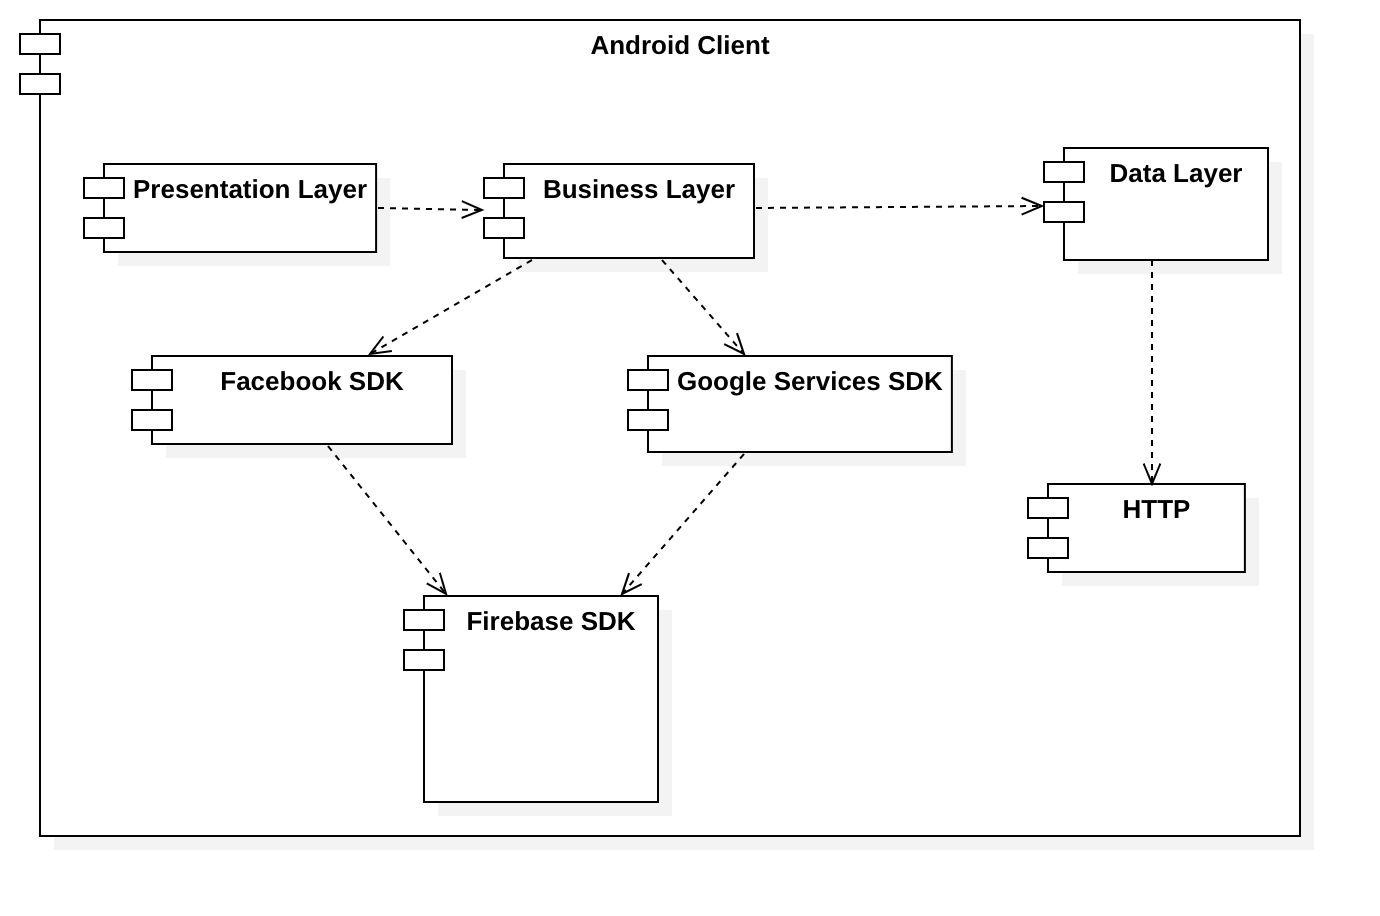
\includegraphics[scale=0.25]{androiddiagram}
  \caption{Android component Diagram}
  \label{fig:android-component}
\end{figure}


\begin{figure}[H]
	\centering
  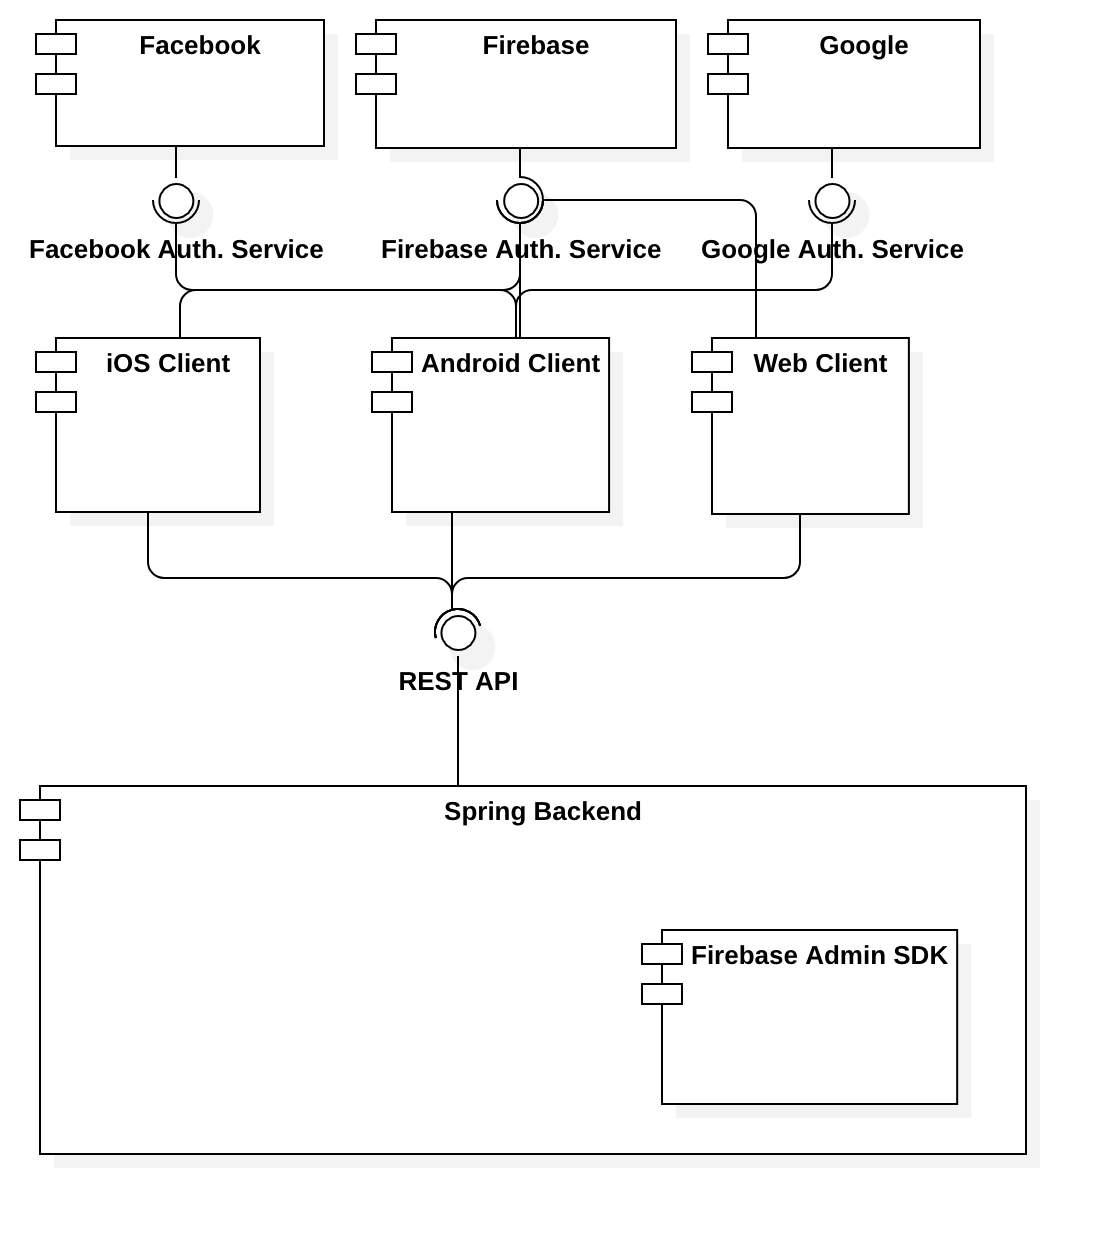
\includegraphics[scale=0.25]{systemdiagram}
  \caption{Component Diagram}
  \label{fig:component}
\end{figure}



\newpage
\section{Domain Description}
 The Class Diagram on Figure \ref{fig:domain} represents the Domain Model of the application, it provides visual representation of Entities and relations between them. The Design is based on the entities used on server-side.

\begin{figure}[H]
  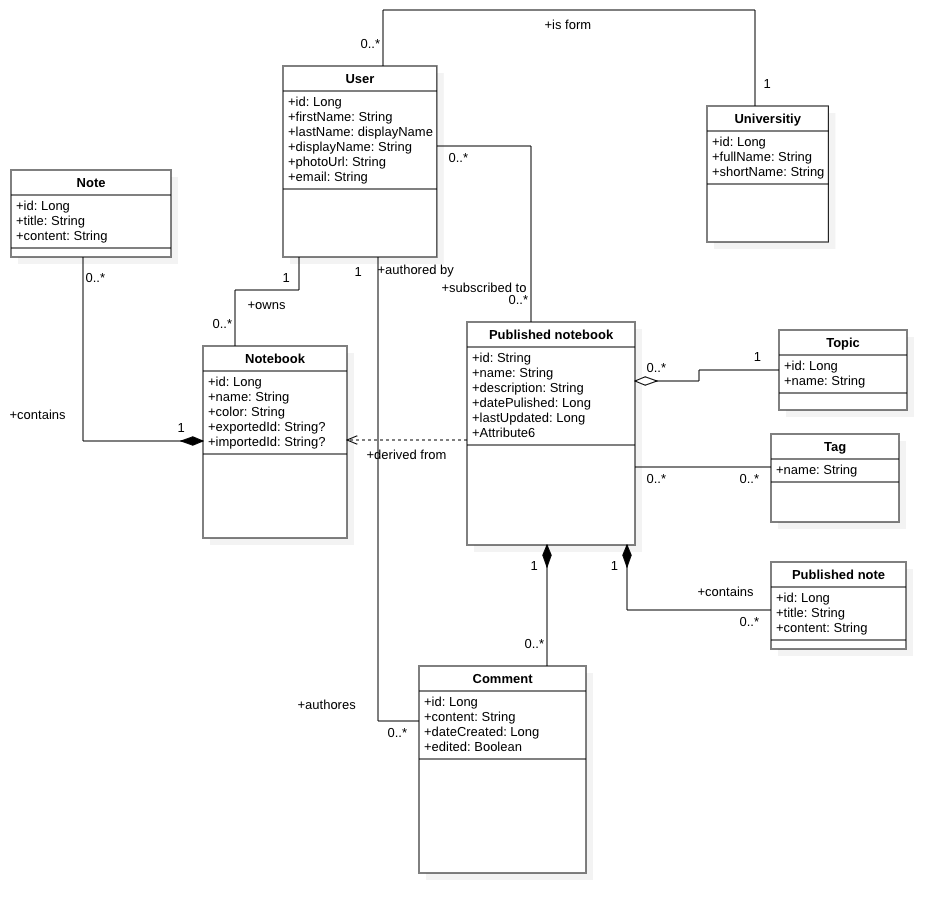
\includegraphics[width=\linewidth]{Domain}
  \caption{Domain Diagram}
  \label{fig:domain}
\end{figure}

 

\subsection{User}
	The User entity represents someone who has completed registration flow using one of the client applications or created manually (in case of Admin role). This entity contains such properties as: role, first name, last name, email address, password, university. Due to the fact, that \appname\ provides several ways for the user to authorise, some of the properties will either come from the user's input or from the 3rd party API (such as Firebase).
	
\subsection{Note}
	Note represents a single piece of information. It consists of two properties: title and content. These can be described as term and definition or question and answer. Each note must be assigned to one of the notebooks, hence there is a 1:N relation.
\subsection{Notebook}
	Notebook is one of the main entities used in the application flow, and  can be created by an authenticated user. The soul purpose of the Notebook is to store Notes and serve as a source for a Published Notebook. Properties name and colour are used to help users distinguish between different Notebooks.
	
	
\subsection{University}
University represents a school, where the User can assign himself as a student during registration flow. It is used to unite users from the same school to make content searching easier. 

\subsection{Published Notebook}
Published Notebook represents a shareable content. It can be created by user, based on one of his/her notebooks by providing some additional details:
name, optional description,  topic and optional list of tags. All these properties are later used in a searching flow to optimise results.

\subsection{Topic}
Topic represents the main topic or subject of the Published Notebook. Topic contains only one property -- its name
\subsection{Tag}
Tag is a short label attached to the Published Notebook. It is mainly  used to narrow the topic or school. Tag has only one property -- its actual value stored as the name.

\subsection{Comment}
Users can comment on published notebooks. Most of the properties are assigned automatically, with the only exception being content: it represents the body of the comment and assigned by the user.


\newpage
\section{Requirements}
It is important to establish all functional and non-functional requirements for \appname. The section bellow contains all requirements designated  before the start of the development.

\subsection{Functional Requirements}
\bigskip
\textbf{User Authentication}
\begin{itemize}
	\item \textbf{F1: Registration/Login using email} Access to \appname\ is possible by creating an account using an email address/password combination.
	\item \textbf{F2: Registration/Login using Facebook} The user will be able to use his/her Facebook account to access \appname.
	\item \textbf{F3: Registration/Login using Google} The user will be able to use his/her Google account to access \appname.
	\item \textbf{F4: Store OAuth token} API Authentication Token will be stored in a device memory.
	\item \textbf{F5: Token refreshment} API Token will be refreshed when needed, so the user will not have to login again.
	\item \textbf{F6: University selection} As part of user registration flow, the user will be able to select his/her university.
	\item \textbf{F7: University Addition} The user will be able to add his/her school, in case of not finding it in a \appname\ database.
\end{itemize}
\bigskip
\textbf{Library Management (Notes \& Notebooks)}
\begin{itemize}
	\item \textbf{F7: Notebook creation} The user will be able to create new notebooks with the name he/she choose.
	\item \textbf{F8: Notebook deletion} The user will be able to delete existing notebooks.
	\item \textbf{F9: Notebook name edition} The user will be able to edit notebooks names.
	\item \textbf{F10: Note creation} The user will be able to create a note with a specific title and content.
	\item \textbf{F11: Note edition} The user will be able to edit an existing note, or completely delete it.
	\item \textbf{F12: Show Notebooks}: The user will be able to view all the notebooks he/she created.
	\item \textbf{F13: Show Notes}: By clicking on notebook item, the user will be able to view the list of notes that are assigned to this notebook.
	\item \textbf{F14: MathJax/ASCII Math support}: User will be able to use complex mathematical expressions as notes content
\end{itemize}

\bigskip
\textbf{Sharing Hub}
\begin{itemize}
	\item \textbf{F15: View published notebooks} The user will be able to view notebooks published by other users.
	\item \textbf{F16: Search through published books} The user will be able to search through the published notebooks by applying different filters (such as author, university, and subject/topic).
	\item \textbf{F17: Browse through published notebook} User will be able to see notes inside the notebook that has been published.
	\item \textbf{F18: View comments} User will be able to view others users comments discussing a notebook that have been published.
	\item \textbf{F19: Leave a comment} The user can comment on an other user published notebook.
	\item \textbf{F20: Delete a comment} The application will allow the user to delete his/her comment.
	\item \textbf{F21: Edit a Comment} The application will allow the user to edit his/her comment
	\item \textbf{F21: Save published notebook} User will be able to save published notebook to his/her library.
	\item \textbf{F22: Publish notebook} User will be able to publish his/her notebook.
	\item \textbf{F23: Update published notebook} The Author of the published notebook will be able to update its information.
	\item \textbf{F24: Delete published notebook} The Author of the published notebook will be able to delete the his/her notebook from shared space.
	\item \textbf{F25: Share notebook} The user will be able to share his/her notebook by generating a deep-link.
	\item \textbf{F26: Notification on update} The user will be notified on updates to the Published notebook they have subscribed to.
	\item \textbf{F27: Suggestions} Subscribers will be able to suggest a change or correction to the Published Notebook. The author will be able to approve it, which will result in the update of the Published Notebook, or decline it.
	\item \textbf{F28: Copy Published Notebook} The user will be able to copy a published notebook. This will create a standalone copy of this notebook in the user's library.
 \end{itemize}

\bigskip
\textbf{Study Hub}
\begin{itemize}
	\item \textbf{F29: Start a Flashcards walkthrough} The user will be able to use an interactive method of looking through his/her notes.
	\item \textbf{F30: Start a written test} The user will be able to participate in a written test based on one of the notebooks to test his/her knowledge.
	\item \textbf{F31: Start a self-check} The user will be able to participate in a quiz challenge that will be based on one of his/her notebooks
	
\end{itemize}


\bigskip
\textbf{Profile}
\begin{itemize}
	\item \textbf{F32: View Profile Information} The user will be able to view his/her profile information such as first name, last name, and  university.
	\item \textbf{F33: Edit Profile Information} The user will be able to edit his/her profile information.
	\item \textbf{F34: Logout} The user will be able to logout from the application.
\end{itemize}


\subsection{Non-functional requirements}

\begin{itemize}
  \item \textbf{N1: Native Android application}  The application will be written using native Android SDK.
  \item \textbf{N2: Android Version} The application minimal SDK version must be low enough to support as many devices as possible and high enough to use most applicable  Android APIs considering other functional and non-functional requirements.
  \item \textbf{N3: Material Design} The application user interface will follow the latest Material design guidelines and best practises.
  \item \textbf{N4: Scalable app architecture} The application's architecture must be scalable and easy testable.
    \item \textbf{N5: App Localisation} The application will be able to adapt to different languages based on user locale.
\end{itemize}


\newpage

\section{Existing solutions}

There are several services out there whose goal is similar to \appname. However, most of those solutions are specialised in language-learning and have limited sharing and/or searching options. Each application/service will be reviewed separately and will include a requirements and main processes comparison. 

Symbols are used in Tables  to indicate  requirement availability in the applications. Symbol on Figure \ref{fig:star} represents the functionality  that is fully supported by the application. Symbol on Figure \ref{fig:starhalf} demonstrates that the given functionality is either limited/incomplete or not working as intended. Lastly, symbol on Figure \ref{fig:starborder} indicates that the given application does not support the requirement.
 
\begin{figure}[H]
\centering
\begin{subfigure}{.3\textwidth}
  \centering
  
\includegraphics[scale=0.2]{ic_star_black_24dp}
  \caption{Present Functionality}
  \label{fig:star}
\end{subfigure}%
\begin{subfigure}{.3\textwidth}
  \centering
  
\includegraphics[scale=0.2]{ic_star_half_black_24dp.png}
  \caption{Limited Functionality}
  \label{fig:starhalf}
\end{subfigure}%
\begin{subfigure}{.3\textwidth}
  \centering
  
\includegraphics[scale=0.2]{ic_star_border_black_24dp.png}
  \caption{Absent Functionality}
  \label{fig:starborder}
\end{subfigure}

\caption{Functionality  Symbols}
\end{figure}



\subsection{StudyBlue}

\textbf{StudyBlue} not only partially shares a name with \appname\ but also a goal and a wide range of features. It is clearly one of the biggest rivals on the market and it is very important to determine what StudyBlue does right and what it does not. How most important \appname\ requirements are compared to the StudyBlue functionality can be seen on Table \ref{tab:studyblue}

Notebooks here are called \textit{decks} and notes are represented by \textit{cards}. Moreover, all decks in StudyBlue are stored in specialised folders named Classes and Interests. Interest, as an entity, not only stores decks, but also unites them by a subject or a topic (e.g. Spanish, Literature). Being a student of the university, the user can also create an Interest that will be connected to his/her school -- Class. Both Interests and Classes are split into two parts: shared space, where the user can find all the decks created by other users, and personal space, where the user can keep the decks he/she has created, saved or copied.


\begin{table}[H]
\caption{\appname\ \& StudyBlue requirements comparison}
\label{tab:studyblue}
\begin{tabular}{|l|c|c|}
\hline
\multicolumn{1}{|c|}{\textbf{Requirements / Application name}} & \multicolumn{1}{l|}{\textbf{StudyPad}} & \multicolumn{1}{l|}{\textbf{StudyBlue}} \\ \hline
F6: University Selection                                       & \present                                & \present                                \\ \hline
F13: Show Notes                                                & \present                              & \limited                                \\ \hline
F14: MathJax /ASCII Math support                               & \present                               & \limited                                \\ \hline
F16: Browse Published Notebooks                        & \present                                & \present                               \\ \hline
F17: Searching Fo Published Notebooks                    & \present                                & \present                               \\ \hline
F18-F21: User Commentaries                                     & \present                                & \absent                                \\ \hline
F27: User Suggestions                                          & \present                                & \absent                               \\ \hline
\end{tabular}
\end{table}

\begin{itemize}
	\item \textbf{Library management:} The main difference in library management comes with the fact that each deck must be associated with an Interest or Class, moreover, it is not possible just to create a deck, the user has to create at least two cards first. Because of that, library management not only includes managing your decks and card, but also interests and classes. Everything the user has saved or created, whether class, interest or a deck can be accessed via \textit{Backpack}.
	\item \textbf{Publishing:} The Publishing process is quite different compared  to what \appname\ is trying to achieve. When creating a deck, the user can choose whether they want to make his/her deck visible for other users in this Class/Interest or to make it private. It is not possible to collaborate on a deck or suggest a change.
	
	\item \textbf{Importing}: As mentioned before, user can save a deck from an existing Interest/Class to their personal space, but they will not be able to make any edits without making a copy.
	\item \textbf{Discovering:} The fact that all decks are either assigned to an Interest or a Class makes searching quite simple. The user can search for deck, classes and users by its name. All these searching options are separated in the UI, so there is no way of combining them. Searching based on the Interest is also available, but the user has to add this Interest to his/her \enquote{Backpack}.
	\item \textbf{UI \&  UX}: StudyBlue has been in development roughly since 2009, and as for now, UI looks outdated and UX can be greatly improved. The most common UI issue here -- Inconsistent usage of UI elements styles.
\end{itemize}

 \subsection{Quizlet}
\textbf{Quizlet} is primarily used for learning languages, from where most of the limitations come from. The closest analogy to a Notebook here is a Study set with Terms inside. Being an application for language learners makes the process of generating different tests and quizzes quite easy, and this is where this application shines the most. Table \ref{tab:quizlet} shows requirements comparison between \appname\ and Quizlet.

\begin{table}[H]
\caption{\appname\ \& Quizlet requirements comparison}
\label{tab:quizlet}
\begin{tabular}{|l|c|c|}
\hline
\multicolumn{1}{|c|}{\textbf{Requirements / Application name}} & \multicolumn{1}{l|}{\textbf{StudyPad}} & \multicolumn{1}{l|}{\textbf{Quizlet}} \\ \hline
F6: University Selection                                       & \present                                & \absent                                \\ \hline
F13: Show Notes                                                & \present                                                                & \absent                                \\ \hline
F14: MathJax /ASCII Math support                               & \present                                                                & \absent                                \\ \hline
F16: Browse Through Published Notebooks                        & \present                                                                & \present                               \\ \hline
F17: Search Through Published Notebooks                    & \present                                                                & \limited                               \\ \hline
F18-F21: User Commentaries                                     & \present                                                                & \absent                                \\ \hline
F27: User Suggestions                                          & \present                                                                & \limited                               \\ \hline
\end{tabular}
\end{table}

\begin{itemize}
	\item \textbf{Publishing}: Similar to StudyBlue, all Study Sets are visible to everyone else by default. However, Quizlet provides a wider variety of privacy options. Study Set can either be completely public, private or semi-private using a password protection. Password protection can also be used to allow certain users to modify a study set.
	\item \textbf{Importing}: Importing flow allows user to either copy or save the study set to a specific folder. This flow may confuse some users, because only copy allows the user to actually add a study set to their library and modify it. Saving study set to the specific folder only saves the link to it and splits library management in two parts.
	\item \textbf{Discovering:} This limitation comes from the fact that Quizlet is an app for studying foreign  languages. As a consequence, the only distinctions between Study Sets are its name and its language. These are the only two options available when searching through study sets.

\end{itemize}

\subsection{Cram}
\textbf{Cram} is very similar to Quizlet but seems highly outdated in terms of UX/UI and brings some sharing limitations to the table. Table \ref{tab:cram} shows a requirements comparison between \appname\ and Cram.



\begin{table}[H]
\caption{\appname\ \& Cram requirements comparison}
\label{tab:cram}
\begin{tabular}{|l|c|c|}
\hline
\multicolumn{1}{|c|}{\textbf{Requirements / Application name}} & \multicolumn{1}{l|}{\textbf{StudyPad}} & \multicolumn{1}{l|}{\textbf{Cram}} \\ \hline
F6: University Selection                                       & \present                                & \absent                             \\ \hline
F13: Show Notes                                                & \present                                & \present                            \\ \hline
F14: MathJax /ASCII Math support                               & \present                                & \limited                            \\ \hline
F16: Browse Through Published Notebooks                        & \present                                & \present                            \\ \hline
F17: Search Through Published Notebooks                    & \present                                & \limited                            \\ \hline
F18-F21: User Commentaries                                     & \present                                & \absent                             \\ \hline
F27: User Suggestions                                          & \present                                & \absent                             \\ \hline
\end{tabular}
\end{table}

\begin{itemize}
	\item  \textbf{Publishing:} Content publishing is similar to Quizlet -- All sets are either visible by other users or not. Sharing a deep-link to a single study set was not functional at the time of writing this section.
	\item \textbf{Discovering}: Searching for content in Cram is even more limited compared to Quizlet, only the name of the study set is used
	\item \textbf{Importing}: Library management here is split in three parts: User personal sets, Favourite sets and Recently studied. When searching, there is no way to save a published study set to a personal library, however, it will be automatically saved to Recent section, or the user can add it manually to Favourites. It is not possible to make any local edits.
\end{itemize}


\subsection{TinyCards}

\textbf{TinyCards} is a flash-card application made the same developer that created Duolingo --  one of the biggest language-learning applications in the market. TinyCard is meant to be more generic as it alows users to create custom study sets, often not limited to languages. Table \ref{tab:tinycards} shows how the \appname\ requirements compare to the TinyCards functionalities.

\begin{table}[H]
\caption{\appname\ \& TinyPads requirements comparison}
\label{tab:tinycards}
\begin{tabular}{|l|c|c|}
\hline
\multicolumn{1}{|c|}{\textbf{Requirements / Application name}} & \multicolumn{1}{l|}{\textbf{StudyPad}} & \multicolumn{1}{l|}{\textbf{TinyCards}} \\ \hline
F6: University Selection                                       & \present                                & \absent                                  \\ \hline
F13: Show Notes                                                & \present                                & \present                                 \\ \hline
F14: MathJax /ASCII Math support                               & \present                                & \absent                                  \\ \hline
F16: Browse Through Published Notebooks                        & \present                                & \present                                 \\ \hline
F17: Search Through Published Notebooks                    & \present                                & \limited                                 \\ \hline
F18-F21: User Commentaries                                     & \present                                & \absent                                  \\ \hline
F27: User Suggestions                                          & \present                                & \absent                                  \\ \hline
\end{tabular}
\end{table}


	\begin{itemize}
		\item \textbf{Importing:} Similar to Cram, it is not possible to edit the study set the user has downloaded and saved to their library
		\item \textbf{Challenges:} Tests are generated automatically and there is no way to choose the test type.
	\end{itemize}



\chapter{Design}
\subsection{Used Components}
This section contains a list of Material Design specific Components (not including widely used elements such as Buttons and Input Fields) used when creating design for \appname.


\begin{itemize}
	\item \textbf{Floating Action Button (FAB)}: According to Material Design Guidelines: \quoting{A floating action button (FAB) performs the primary, or most common, action on a screen. It appears in front of all screen content, typically as a circular shape with an icon in its center.} \cite{material-fab} FAB is widely used in creating content, hence it found its place in the note-taking part of the application.
	\item \textbf{Bottom App Bar}: \quoting{Bottom app bars provide access to a bottom navigation drawer and up to four actions, including the floating action button.} \cite{material-bottomappbar}. In \appname\ it is primarily used in the details screens with one primary action (FAB) and two or more secondary actions.
	\item \textbf{Chips}: \quoting{Chips are compact elements that represent an input, attribute, or action.}\cite{material-chips}. In \appname\ it is used mainly for displaying Tags and in Searching flow. In most of the cases it will be placed in the ChipGroup -- a special container to store dynamic amount of Chips
	\item \textbf{Bottom Sheets}: \quoting{Bottom sheets are surfaces containing supplementary content that are anchored to the bottom of the screen.}. The most common Bottom Sheet type used in \appname\ is Modal Bottom Sheet, that allows user to provide certain kind of input, like Topic, Univerisity selection e.t.c
	\end{itemize}

\section{UI \& UX}

This section contains most important screens description from UI \& UX standpoint, wireframes and it's iterations

\subsection{Library Managent}
Library management requirements (F7-F14) are covered by the first top-level destination: \textbf{My Library}. This part of the application serves as the main entry point for the returning users. Wireframes of this sections can be viewed on Figure \ref{fig:section-library}.
	
	Its first screen, as shown on Figure \ref{fig:notebooks}, contains a scrollable list of Notebooks and provides access to the various notebook-management related actions such as: Notebook creation(triggered by FAB), edition, deletion and sharing
		
	By clicking on one of the notebooks in the list, user will be transferred to the Notes List Screen (Figure \ref{fig:notes}). Similar to Notebooks List Screen, this screen contains a scrollable list of notes from this notebook and  covers all the note management related actions and interactions such as Note creation, edition and deletion. Once again, FAB is used for to trigger create action.
	
	Finally, by choosing a note, the user will be able to view its details. As shown of Figure \ref{fig:detail}, this screen utilises Bottom app bar to provide access for key actions and FAB.
	
\begin{figure}
\centering
\begin{subfigure}{.5\textwidth}
  \centering
  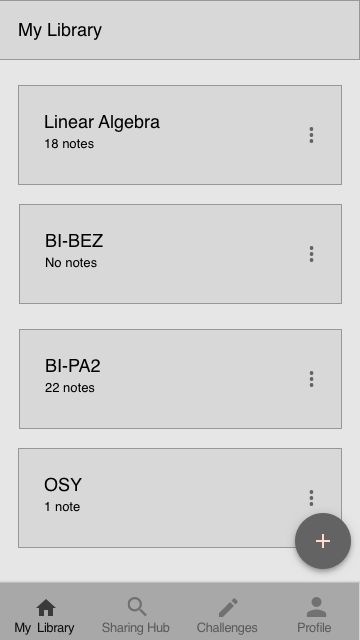
\includegraphics[scale=0.4]{Notebooks.png}
  \caption{Notebooks List Screen}
  \label{fig:notebooks}
\end{subfigure}%
\begin{subfigure}{.5\textwidth}
  \centering
  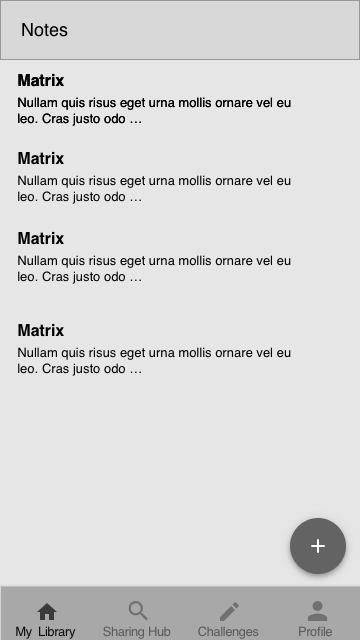
\includegraphics[scale=0.4]{Notes}
  \caption{Notes List Screen}
  \label{fig:notes}
\end{subfigure}
\begin{subfigure}{.5\textwidth}
  \centering
  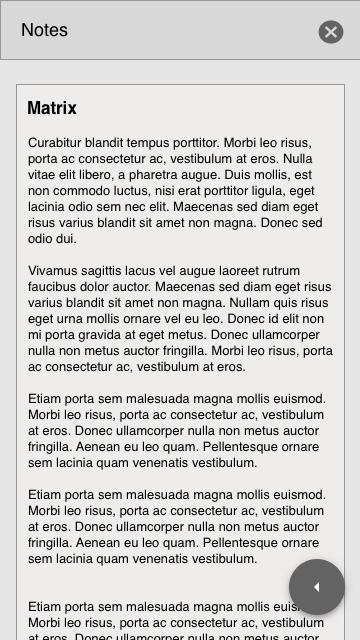
\includegraphics[scale=0.4]{NoteDetailView}
  \caption{Note Detail Screen}
  \label{fig:detail}
\end{subfigure}

\caption{My Library Section Wireframes}
\label{fig:section-library}
\end{figure}

\newpage
\subsection{Notebook Publishing}
The fact the all the content in \appname\ is made by its community makes Notebook Publishing Flow is one of the core functionalities of the application. The flow it self acts as complex form with different types of inputs:
\begin{itemize}
	\item Notebook name -- Single-line input field, will be pre-filled with the name of local Notebook that is being published.
	\item Language of the Notebook -- Selector, will be pre-filled with the current user locale.
	\item University/School associated with this Notebook -- Selector, will be pre-filled with the User's university, this field is optional.
	\item Topic/Category of the Notebook -- Selector, this field is mandatory
	\item Tags -- ChipGroup, chosen tags will be represented by Chips. The field is optional
	\item Description/Message for other users -- Multi-line input field, this field is optional.
\end{itemize}



Considering an amount of input needed, its variety, the decision was made to split this form into several steps. It will allow make the form more dynamic and put more emphasis on some inputs by grouping them.

First step will include all fields that can be pre-filled: Notebook's name, language and University. This will allow to skip this step in most cases, making it only about controlling pre-filled information.
Second step will require users to provide search-relevant information, such as Tags and Topic/Category, topic being a required option. Third step will allow user to provide a message or a more detailed of description of the Notebook. Fourth step will be all about confirmation, in which the user can double-check information he/she entered and submit it.

Though the choice of UI elements in different steps is well defined, they way we present these steps is not. Simplified wireframes with different approaches of how the steps can be presented are shown on Figure \ref{fig:publishing-sketches}. In the end, decision to go with the Stepper solution was made as it gives a number of advantages:
	\begin{itemize}
		\item Stepper is a standardised element of Material Design
		\item In every step, Stepper gives an overview of all steps available and its completion state
		\item Stepper allows to quickly navigate between different steps.
	\end{itemize}
	
	More detailed wireframes for this flow using Stepper are shown of Figure \ref{fig:publishing-wireframe}

\begin{figure}
\begin{subfigure}{.5\textwidth}
  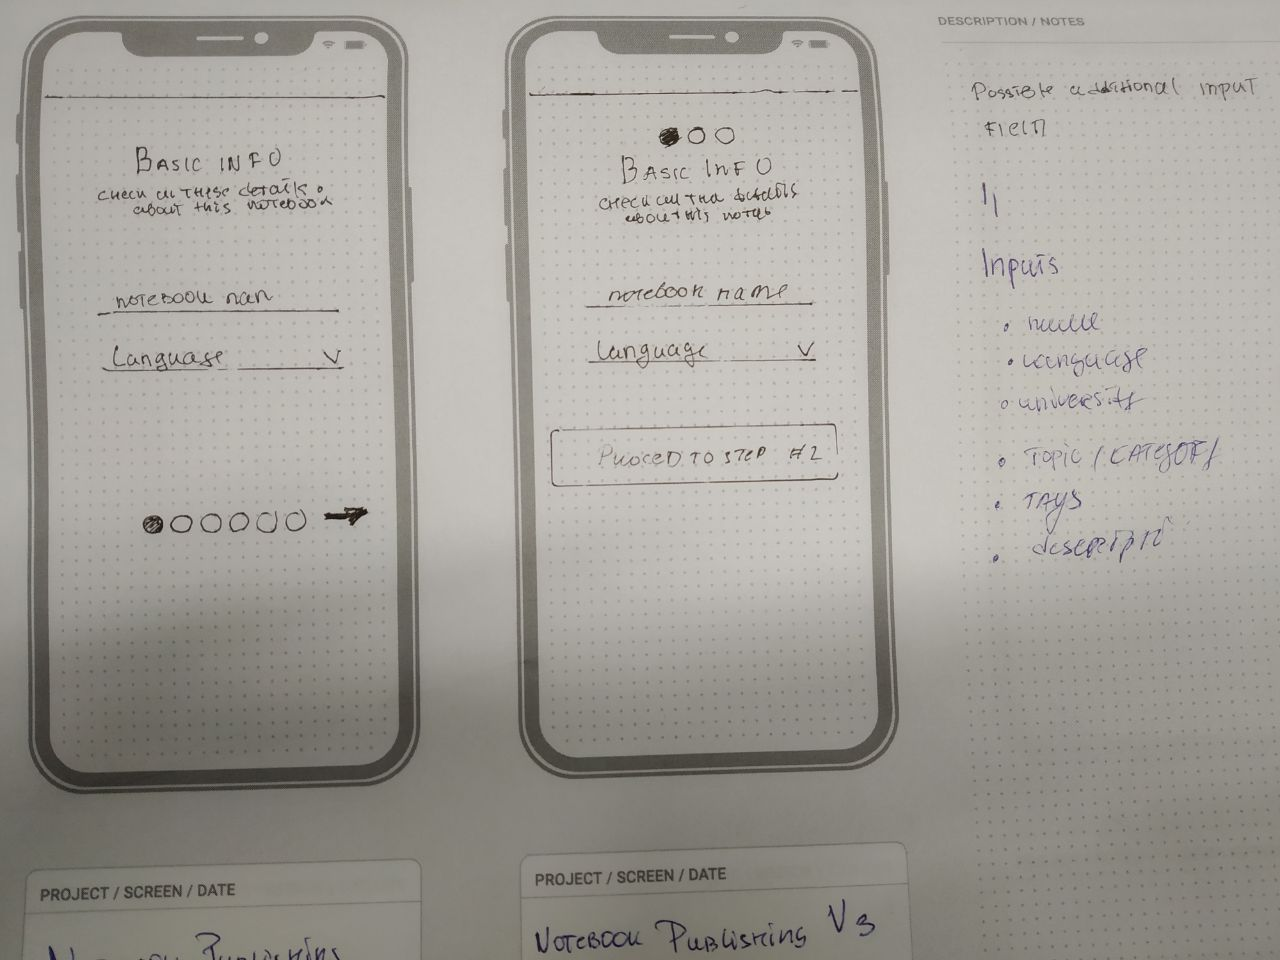
\includegraphics[scale=0.3]{publishing-sketches}
\end{subfigure}%

\begin{subfigure}{.5\textwidth}
  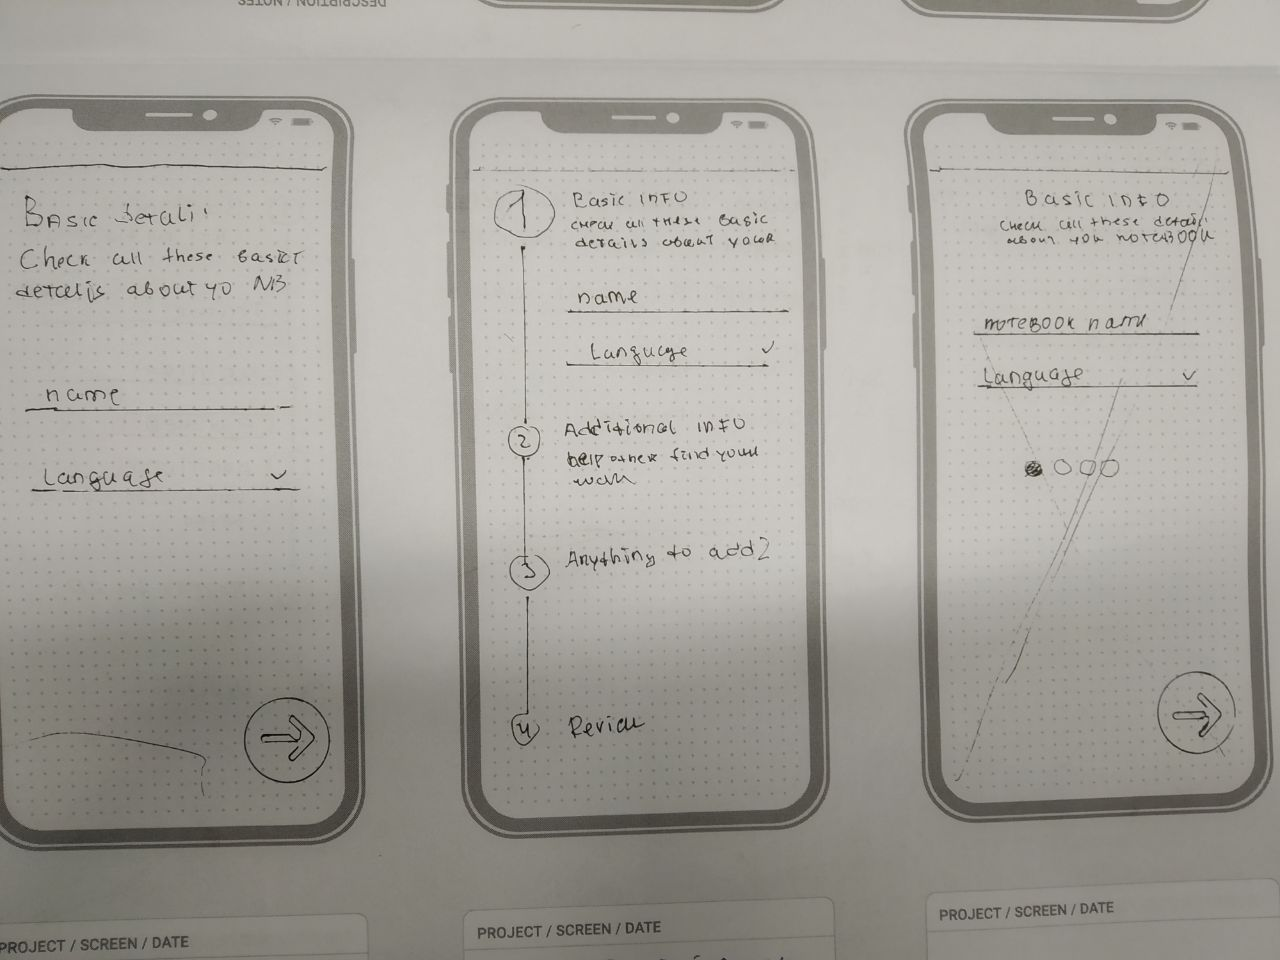
\includegraphics[scale=0.3]{publishing-sketches2}
\end{subfigure}

\caption{Notebook Publishing Flow - Sketch Phase}
\label{fig:publishing-sketches}
\end{figure}


\begin{figure}
\centering
\begin{subfigure}{.5\textwidth}
  \centering
  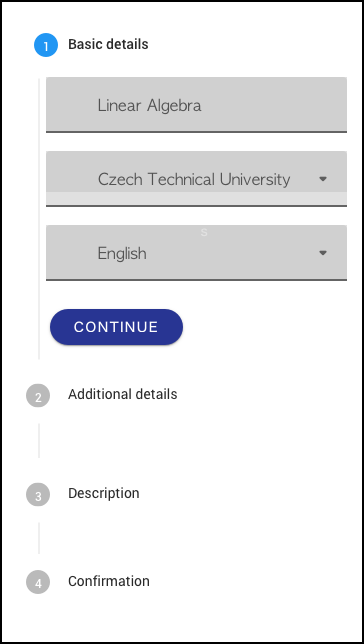
\includegraphics[scale=0.4]{step1}
  \caption{First Step of Notebook Publishing}
  \label{fig:step1}
\end{subfigure}%
\begin{subfigure}{.5\textwidth}
  \centering
  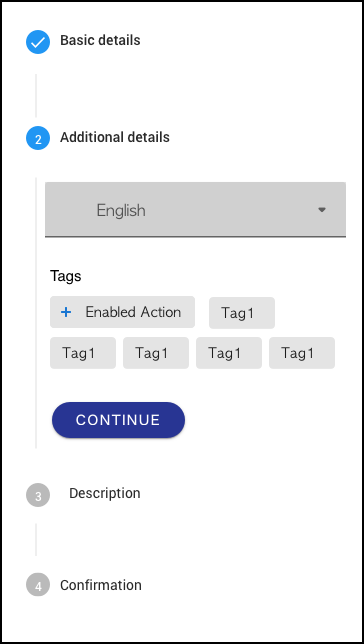
\includegraphics[scale=0.4]{step2}
  \caption{Second Step of Notebook Publishing }
  \label{fig:step2}
\end{subfigure}
\begin{subfigure}{.5\textwidth}
  \centering
  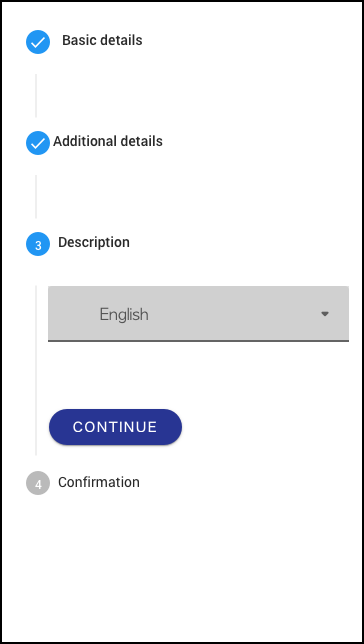
\includegraphics[scale=0.4]{step3}
  \caption{Third Step of Notebook Publishing }
  \label{fig:step3}
\end{subfigure}

\caption{Notebook Publishing Wireframes}
\label{fig:publishing-wireframe}
\end{figure}




\subsection{Sharing Hub}

\textbf{Sharing Hub} is another top-level destination, that allows users to access various Notebooks published by other users.

In the early stage of the \appname\ development, Sharing Hub root screen (Figure \ref{fig:section-sharinghubv1}) contained only one list with the Published Notebooks, with the idea of showing the most recently added Notebooks. Later on, the decision was made to make this screen more personalised by introducing Sections and Notifications preview (Figure \ref{fig:section-sharinghubv2sletch}).


Section is a small list of Published Notebooks of fixed size, that can be scrolled horizontally. By introducing these small lists it will be possible to group Published Notebooks into personalised sets (Notebooks from the user's university for example). Each Section is result of an executed query, so it can be used to facilitate the search flow. So, clicking the See All Button, will launch Search Flow with pre-filled search options, associated with this section.

Another newly added element is a Notifications preview. Located on the top part of the screen, this element displays notifications about the most recent activities like Notebooks updates. By clicking the notification user will be to view the Notebook details associated with this notification.


\begin{figure}[H]
\centering
\begin{subfigure}{.5\textwidth}
  \centering
 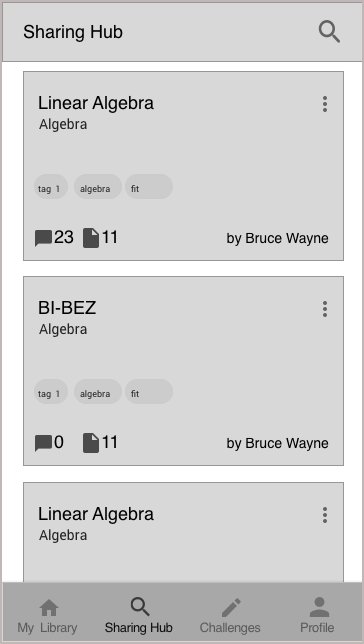
\includegraphics[scale=0.4]{SharingHub}
  \caption{Landing page v1}
  \label{fig:section-sharinghubv1}
\end{subfigure}%
\begin{subfigure}{.5\textwidth}
  \centering
  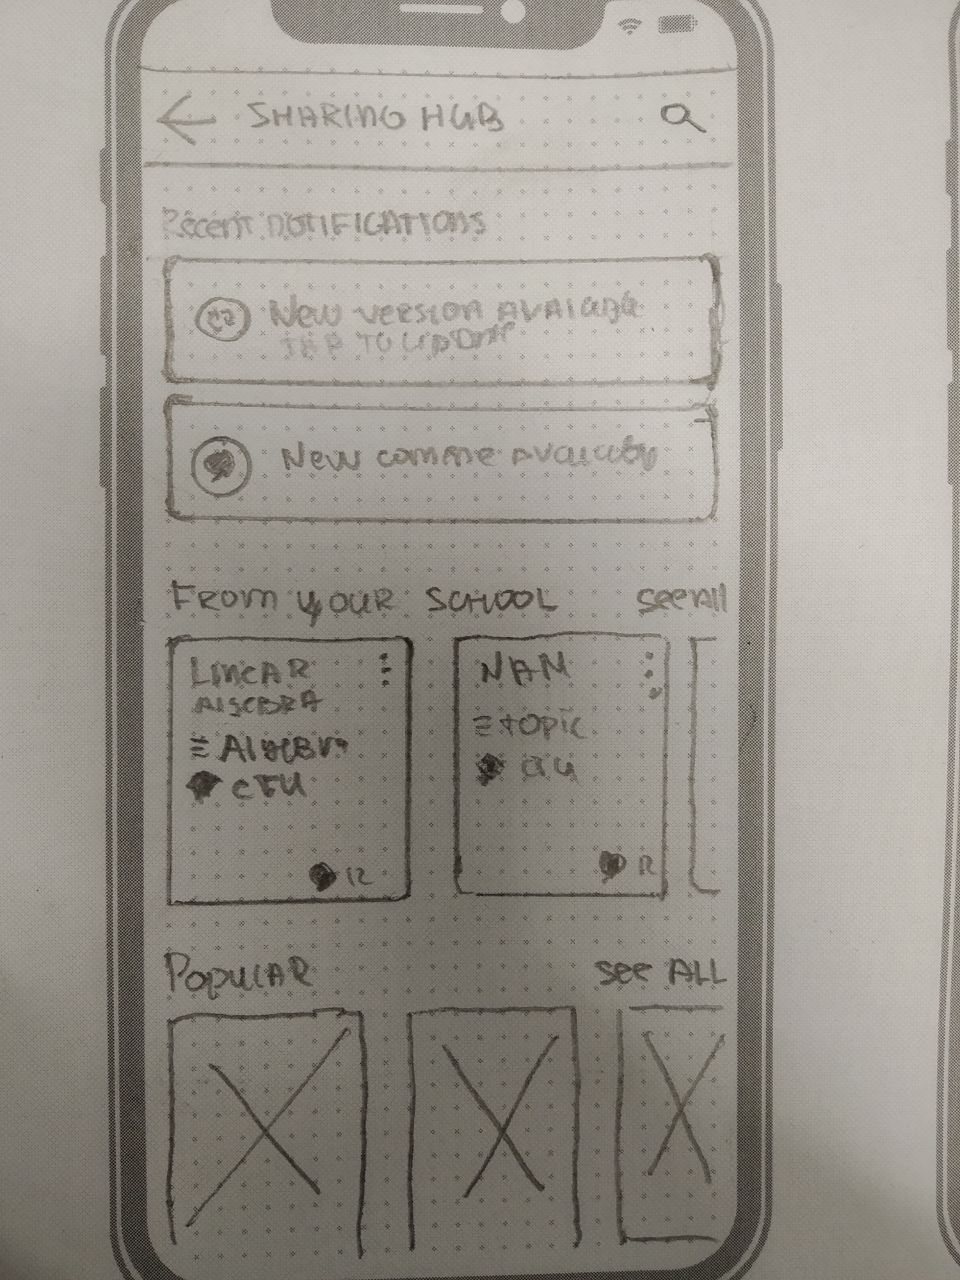
\includegraphics[scale=0.2]{sharingHubV2.jpg}
  \caption{Landing Page v2}
  \label{fig:section-sharinghubv2sletch}
\end{subfigure}

\caption{Sharing Hub Wireframes}
\label{fig:publishing-wireframe}
\end{figure}


\newpage
\subsection{Searching Flow}
 One of the main responsibilities of this screen is to start Search flow. Search flow is either launched by a Search Menu Item located in the Top bar or by the expanding on expanding on the Notebooks Section. Here a list of some basic requirements while
 \begin{itemize}
 
 \item There are should several primary searching/filtering options available: Notebooks name, University/School, Topic/Category and Tags.
 \item All these options must be easily accessible with the idea that more searching options might be introduced during later phases of development.
 \item When none of searching options are active, empty state must be presented.
  \end{itemize}

The resulting wireframe is shown on Figure \ref{fig:section-search} . This approach is using Top App bar to display active searching options. Each options is represented by Chip action, that can have two states: Chip is either inactive  and displays the name of the search option, or it is active, displaying selected option's values. When there are a lot of values selected, in case of multiple Tags for example, last three selected will be shown. 

Clicking the Chip will result in showing Modal Bottom Sheet, that will allow user to tweak selection of the active values and every change to a Search options values will result in updating the search results. Search results themselves appear in the scrollable list bellow the Top Bar. 
   

\begin{figure}[H]
\centering
  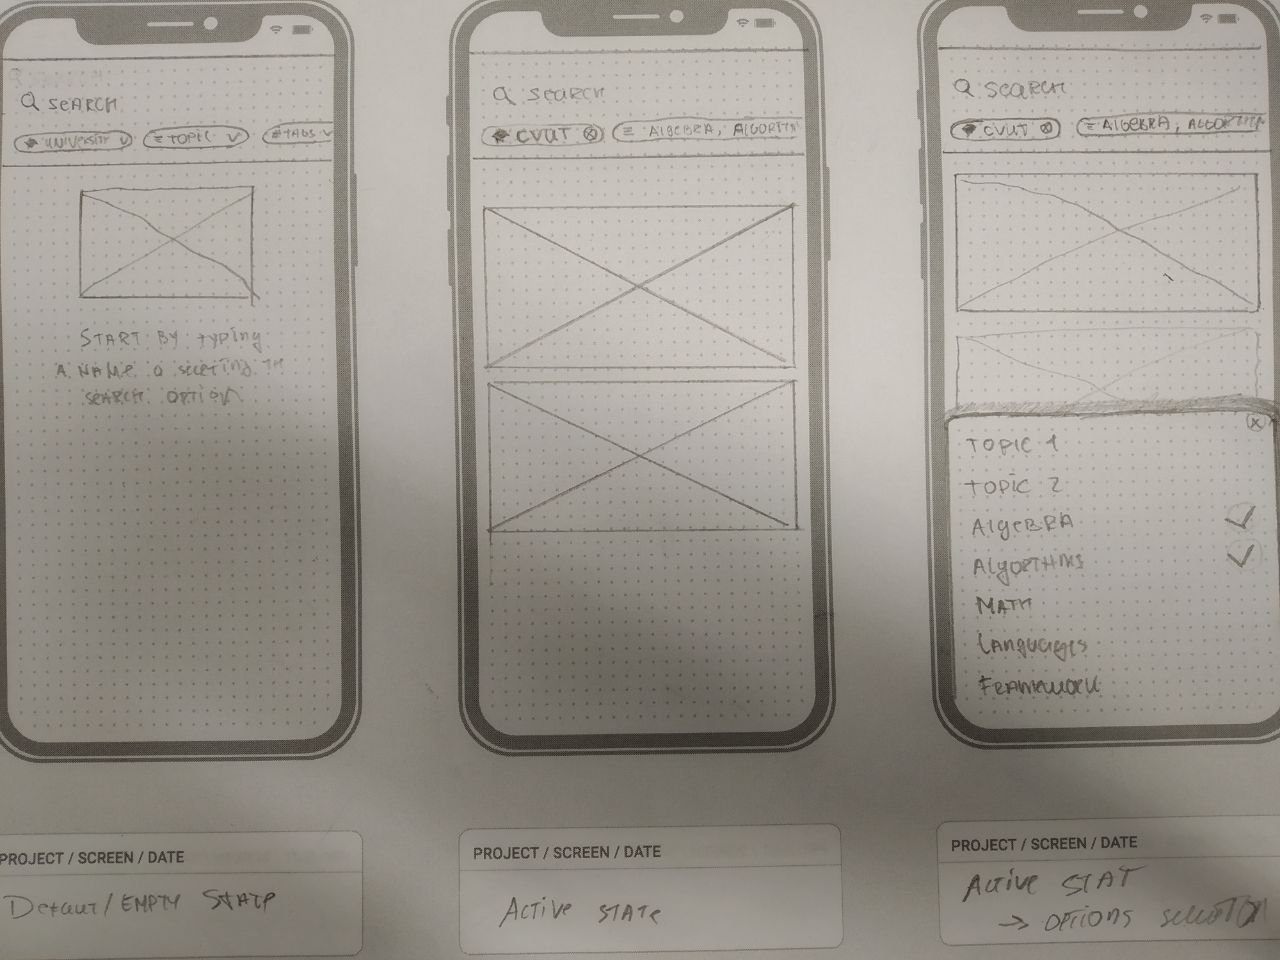
\includegraphics[scale=0.23]{sectionSearch}
  \caption{Search Flow Wireframes}
  \label{fig:section-search}
\end{figure}



 
\subsection{Published Notebook Details}
Published Notebook, as an entity, contains a large amount properties and there are a lot of actions associated with it. This screen will cover all actions regarding user comments (requirements F18-F21) and various Published Notebook actions such as saving, sharing, and copying. Including all these actions and flows into one screen would make UI very crowded, resulting in bad UX. \textit{Tabs} can help solve this issue quite easy.

According to Material Design Guidelines, Tabs can organise content across different screens, data sets, and allow navigation between groups of content that are related and at the same level of hierarchy. \cite{material-tabs}. By using Tabs, this screen can be split into two distinct sections: Detail Tab and Comments Tab, thus dividing responsibilities and making this screen more responsive.
 

Details Tab (Figure \ref{fig:published-details}) features key details about this Notebook. Due to the fact that there are a lot of details to display, all the properties are  divided into several groups.

\begin{itemize}
	\item \textbf{Basic details}: This group contains simple properties such as Notebook's name, its author, category/topic, language and associated university.
	\item  \textbf{Description}: This group contains more dynamic content such as description, that can take multiple lines, and a Chip Group with tags.
	\item \textbf{Notebook Action:} This view represents a primary action available for this notebook in regards to user Library. This can either act as a Save button, that will save the latest Notebook version to the users Library or as an Update Button, that will result in applying changes from local notebook to the Published one, thus updating its contents. If none of the actions are available, this view will be hidden.
	 \item \textbf{Suggestions}: This view group serves as preview and an entry point for suggestions left by other users. 
	\item \textbf{Notes Preview}: Last view at the bottom of the screen serves as an entry point for notes browsing.
\end{itemize}
 
Comments tab, as shown on Figure \ref{fig:published-comments}, contains a scrollable list of the user comments and an Input Field, that will be used to create a new comment, or edit the old one. Also, every comment contains an options button that will trigger either an edit or a delete action.

\begin{figure}[H]
\begin{subfigure}{.5\textwidth}
  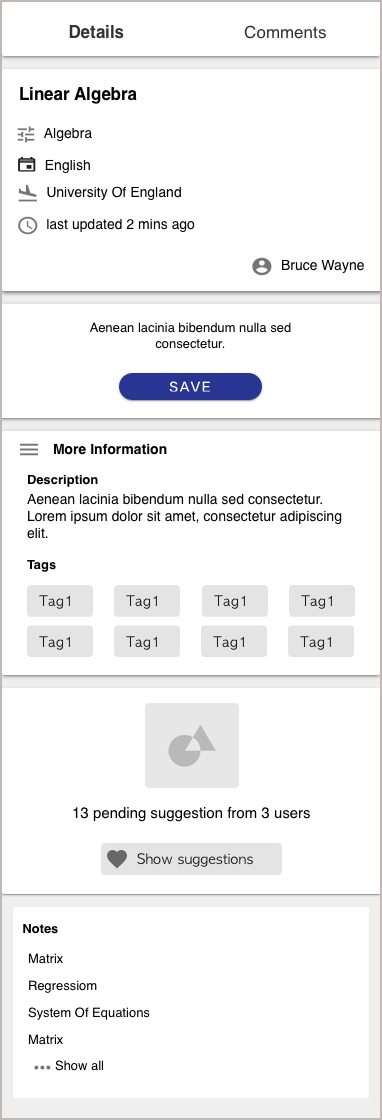
\includegraphics[scale=0.45]{comments}
  \caption{Details Tab}
  \label{fig:published-details}
\end{subfigure}%
\begin{subfigure}{.5\textwidth}
  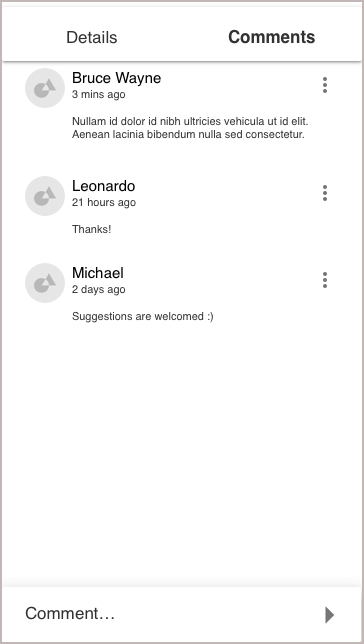
\includegraphics[scale=0.5]{details}
  \caption{Comments Tab}
  \label{fig:published-comments}
\end{subfigure}
\caption{Published Notebook Details Wireframes}
\label{fig:section-published}
\end{figure}

\subsection{Challenges}
Current iteration of \appname provides a small amount of very straightforward challenges (or tests) where user can test his/her knowledge of of one of the notebooks. \textbf{Challenges} section serves as an entry point for setting up these different tests.



Its landing screen (Figure \ref{fig:challenge-start}) features a list of recently completed challenges, including some statistics if available,  and three buttons, that are responsible for launching three distinct challenges with add: Flashcards, Write and Self-check. There is also a button that will navigate the user to a more in-depth configuration of his/her trial - Setup Challenge screen. Clicking one of the recently completed challenges entries will launch this challenge with all the options pre-set automatically. If the user hasn't completed any challenge yet, the empty view will be featured.





Besides choosing the type of the challenge and the notebook, Setup Challenge screen (Figure \ref{fig:challenge-setup})  allows the user to select some additional options before generating his test such as order of the question and what will serve as an answer (either title of the note or its content). After all the details required are provided, most importantly challenge type and the notebook, the user will be able to start his test.



Flashcard challenge is one of the simplest tests and requires no validation. Wireframe of this challenge can be seen in Figure \ref{fig:challenge-flash}.  This challenge is just an interactive way to walk through the notes, featuring a scrollable list of notes. User can flip the displayed flashcard to show the answer to a question and back. Navigation here doesn't have any boundaries so that the user can scroll this in any direction.  When reaching the end of the list, the user will see how many notes he/she studied.


Just like the Flashcards challenge, next test features a list of questions base on of the users' notebooks. The idea of Self-check challenge \ref{fig:challenge-self} is straightforward. Given a list of questions, the user must ask himself a simple question: Do I Know the answer? Two buttons below the flashcard are then self-explanatory: It's the user answer, either he/she know the answer or not. Clicking will "I know" will reveal the next question and clicking "Study again" will reveal the answer to the current question.



Write challenge (Figure \ref{fig:challenge-write})  is very similar to the Self-check challenge with the only distinction being that the user must provide his answer using an input field.
His answer will then be validated, and, depending on how close user was to the correct answer, it will either show next question or will require the user to re-submit his answer, correcting his/her mistake.

\begin{figure}[H]
\centering
\begin{subfigure}{.5\textwidth}
  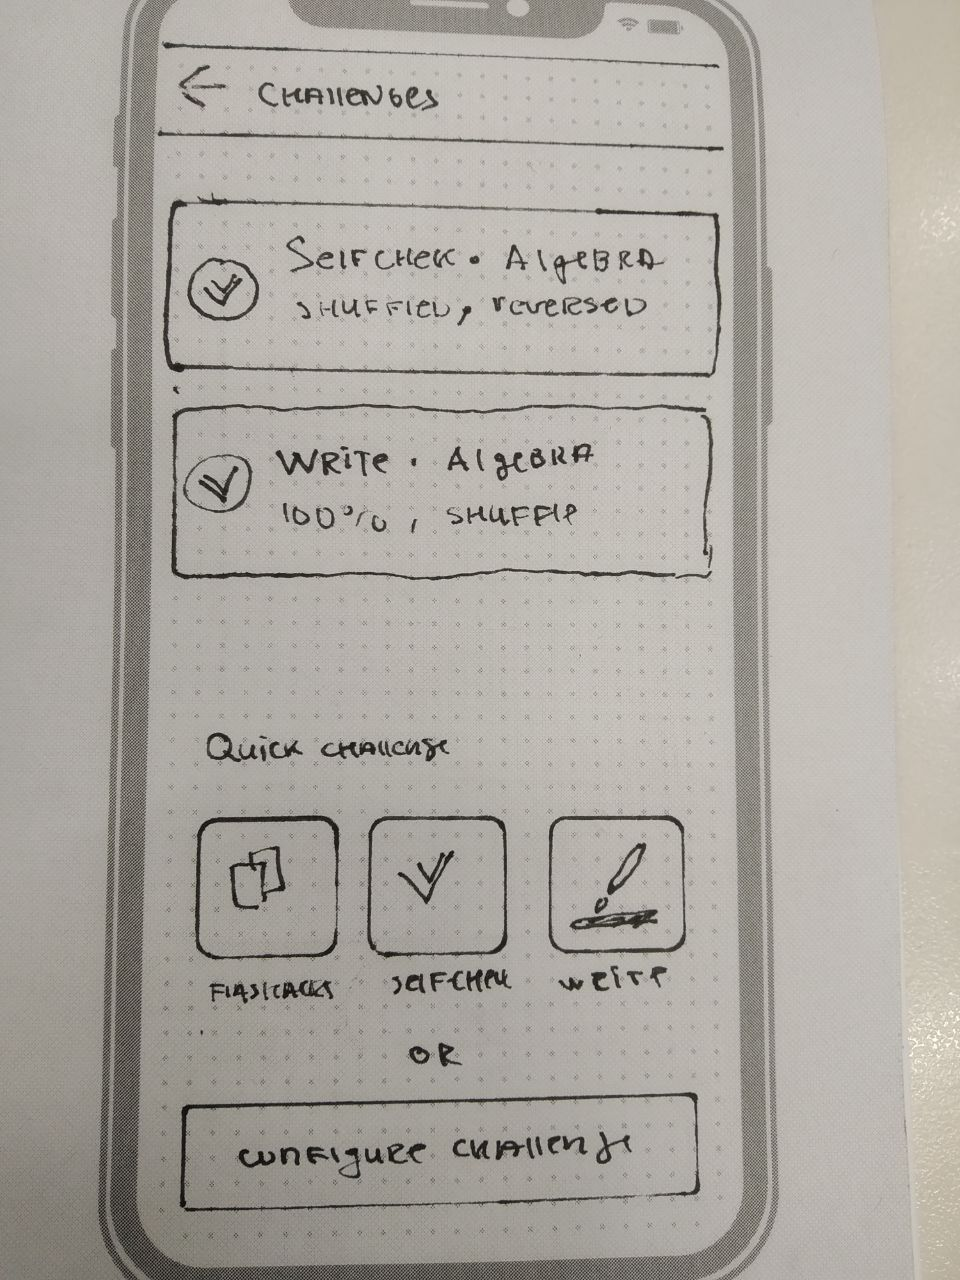
\includegraphics[scale=0.2]{challengesStart}
  \caption{Challenges Landing Screen Wireframe}
  \label{fig:challenge-start}
\end{subfigure}%
\begin{subfigure}{.5\textwidth}
  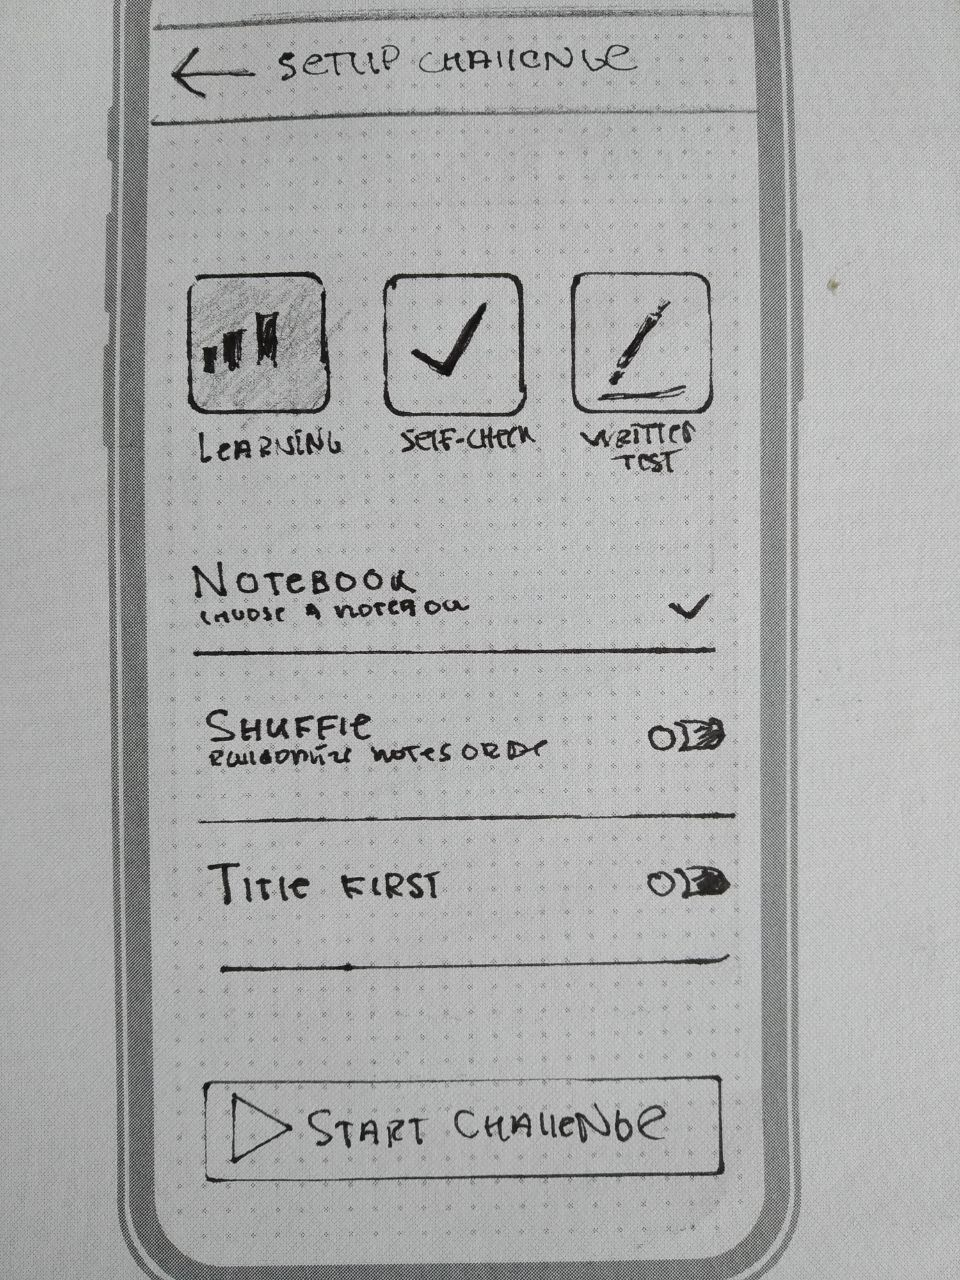
\includegraphics[scale=0.2]{challengesSetup}
  \caption{Setup Challenge Wireframe}
  \label{fig:challenge-setup}
\end{subfigure}
\end{figure}

\begin{figure}[H]
\centering
\begin{subfigure}{.5\textwidth}
  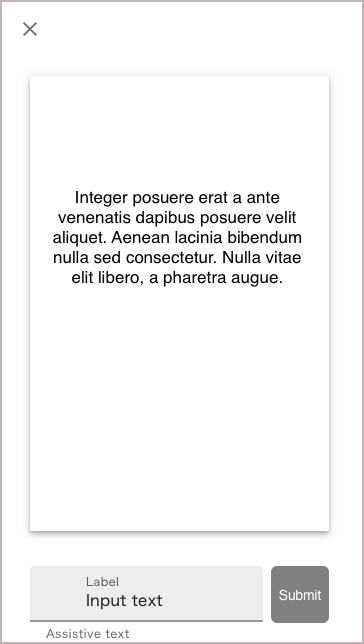
\includegraphics[scale=0.45]{write}
  \caption{Write Challenge Wireframe}
  \label{fig:challenge-write}
\end{subfigure}%
\begin{subfigure}{.5\textwidth}
  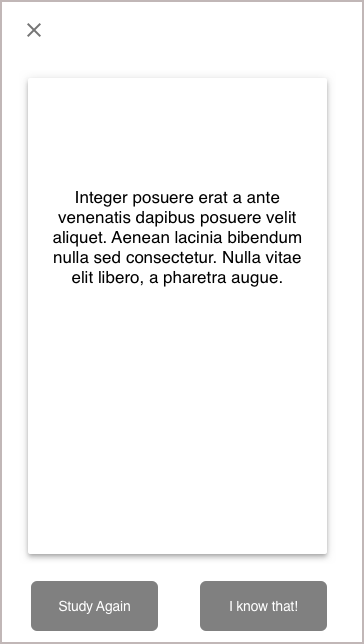
\includegraphics[scale=0.45]{selfcheck}
  \caption{Self-check Challenge Wirefram}
  \label{fig:challenge-selfcheck}
\end{subfigure}
\begin{subfigure}{.5\textwidth}
  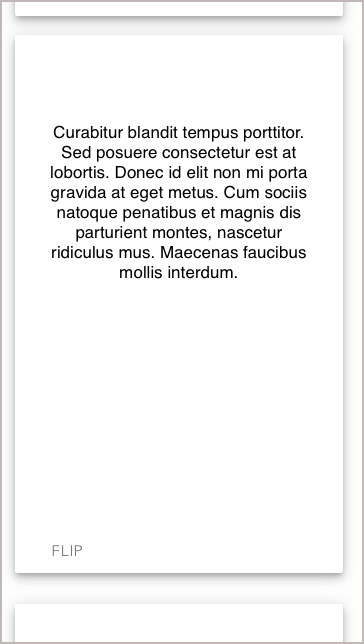
\includegraphics[scale=0.45]{flashcards}
  \caption{Flashcards Challenge Wireframe}
  \label{fig:challenge-flash}
\end{subfigure}
\end{figure}


\subsection{Profile}

\textbf{Profile} is the last top-level destination available from the Navigation bar. As shown on Figure \ref{fig:section-profile}, it features basic information about currently logged-in user and provides buttons to access three more subsections: Profile Edition, Notifications and Settings.

Profile edition screen (Figure \ref{fig:section-editprofile}) allows user to change his/her name and university. Screen contains two input fields, that will be automatically populated with user information, and a Save button, that will only be enabled if one of the input field changes. Pressing Save button will try to update information and navigate back to profile screen in case of success.

Notifications screen contains a scrollable list of  all previously received notifications. It is the same component used in the Sharing Hub screen.

Settings screen contains application-relevant information and preferences. On of the key functionalities here is a Logout button (requirement F34).


\begin{figure}[H]
\begin{subfigure}{.5\textwidth}
  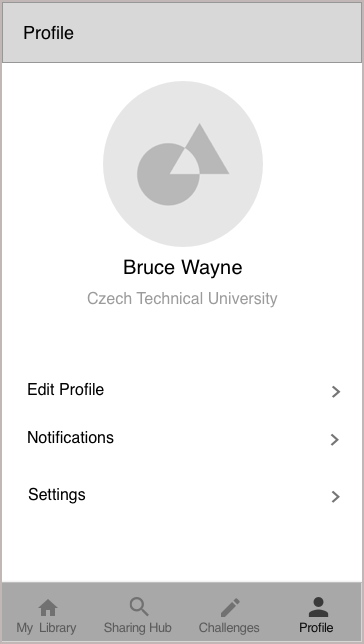
\includegraphics[scale=0.45]{profile}
  \caption{Profile Screen Wireframe}
  \label{fig:section-profile}
\end{subfigure}%
\begin{subfigure}{.5\textwidth}
  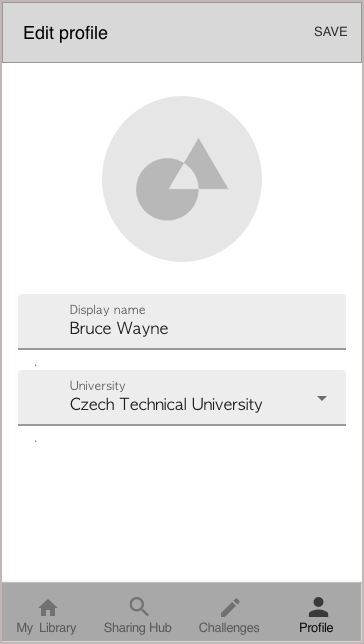
\includegraphics[scale=0.45]{editProfile}
  \caption{Edit Profile Screen Wireframe}
  \label{fig:section-editprofile}
\end{subfigure}
\end{figure}


\section{Application architecture}
On the of key requirements for \appname\ development is its architecture scalability. This section describes the approach chosen for its development and patterns in use

\subsection{MVVM}
MVVM architecture was a rather easy choice for main architecture pattern. It is well supported by Android libraries and recommended by Google. ViewModel serves as glue between Presentation Layer and Data Layer. In example provided by Google (Figure \ref{fig:architecture-final}) Fragments/Activities represents the Presentation Layer and Repository acts as the data layer.


\subsection{Repository}
Repository is an abstraction that deals with the Entities. Repository can have one or multiple data sources. One of the main \appname\ data sources is its REST API. In-memory database will act as a secondary data source to allow some offline capabilities. 

\subsection{Interactors}
Though the repository pattern is a great abstraction for data layer, it would make sense to go even further and apply more Clean architecture principles. Interactor, or a Use-case, is another abstraction that represents single use-case -- one rule of business logic. Interactor is usually talks to the repository and the returns the result to whatever called it in the first place.

This will even more propagate the separation of concerns as every Interactor will only deal with one particular functionality, which will make code more readable and make uni-testing easier in the future.


\subsection{Dependncy Injection}
Dependency injection (DI) is another technique that will help provide a more clean code and will be great help when providing a test-coverage.

\subsection{\appname\ Architecture}
Overall architecture will include following components:
\begin{itemize}
	\item \textbf{Presentation Layer}, that is represented by \texttt{Fragments} and \texttt{Activities}. They are only aware about how to display information and does not contain any complex logic. All the interactions are getting handled by Domain Layer
	\item \textbf{Business Layer} is represented by \texttt{ViewModel}. ViewModel is injected into the Presentation Layer, it handles all user interactions and decides what and when to display, including navigation. ViewModel also executes Interactors and handles its result.
	\item \textbf{Data Layer} is represented by Interactors and Repositories. Interactors get injected into ViewModel and serves to execute certain request in the background and provide a result via callbacks. Repositories provide Entity-based operations using the data sources.
\end{itemize}
 
\chapter{Implementation}
This chapter describes main pin points of \appname\ implementation, platform-specific technologies and libraries. 
\section{Choice of technologies}
\section{Component diagram}
\section{Installation}

\chapter{Testing}


\setsecnumdepth{part}
\chapter{Conclusion}

The goal of this thesis was to develop a StudyPad client for Android OS, which involved domain, requirements and existing solutions analysis as the first step. Next, the application UI and architecture was designed to support the requirements established in the previous step. Finally, the application was developed applying best practices from the world of the modern Android application development.
All requirements specified in the Analysis were implemented along with the  couple new functionalities that were not a part  of the requirements specifications:
\begin{itemize}
	\item A screen to view latest notifications received.
	\item Introduction of real-time features when receiving.
push-notifications when the application is in the foreground.
	\item The functionality that allows users to send feedback about the application.
	\item Offline functionality that covers Challenges and Local Notebooks.
\end{itemize}

The application has not been uploaded to the Play Store yet; hence it has not been tested by the broader set of users.
Testing the application will be the last step to this thesis and it will give me more insight into what was done right and can be improved in the future.

\subsection{Future development}
\appname\ development is far from over.  The current iteration of the application had an emphasis on content creation, sharing, and collaboration, with just a few tests available for users to study and learn. The real process of studying has yet to be researched and executed.
This could be a main focus for the future development of \appname.


There also some small changes that could be  addressed such as:
\begin{itemize}
	\item Powerful Notes editor that would make notes creation easier.
	\item Implementing of Paging. Currently, neither API or the Application supports paging. Paging would improve loading time, which is especially important when there is a lot of content available.
	\item Unit and Instrumentation tests to ensure application stability.
	\item Implementation of Modular Architecture. It would enhance the quality of code and make test coverage easier.
	\end{itemize}
	
	\noindent Though there are still a lot of work to be done on the Android application, \appname\ could be much bigger. In the long run, the iOS client could be finalised, and the Web client implemented making it a fully cross-platform experience. 

\bibliographystyle{iso690}
\bibliography{mybibliographyfile}


\setsecnumdepth{all}
\appendix

\chapter{Acronyms}
% \printglossaries
\begin{description}
	\item[GUI] Graphical user interface
	\item[XML] Extensible markup language
	\item[FAB] Floating Action Button
	\item[UI] User Interface
	\item[UX] User Experience
	\item[FCM] Firebase Messaging Service
	\item[GCM] Google Messaging Service
	\item[DSL] Domain Specific Language
	\item[DI] Dependency Injection
	\item[IoC] Inversion of Control
\end{description}


\chapter{Contents of enclosed CD}

%change appropriately

\begin{figure}
	\dirtree{%
		.1 readme.txt\DTcomment{the file with CD contents description}.
		.1 exe\DTcomment{the directory with executables}.
		.1 src\DTcomment{the directory of source codes}.
		.2 wbdcm\DTcomment{implementation sources}.
		.2 thesis\DTcomment{the directory of \LaTeX{} source codes of the thesis}.
		.1 text\DTcomment{the thesis text directory}.
		.2 thesis.pdf\DTcomment{the thesis text in PDF format}.
		.2 thesis.ps\DTcomment{the thesis text in PS format}.
	}
\end{figure}

\end{document}
